\documentclass[10pt,journal,compsoc,twoside]{IEEEtran}
\IEEEoverridecommandlockouts
% The preceding line is only needed to identify funding in the first footnote. If that is unneeded, please comment it out.
\usepackage{adjustbox}
\usepackage{algorithmic}
\usepackage{amsmath,amssymb,amsfonts}
\usepackage{array}
\usepackage{cite}
\usepackage{colortbl}
\usepackage{gensymb}
\usepackage{graphicx}
\usepackage{makecell}
\usepackage{multirow}
\usepackage{stfloats}
\usepackage{textcomp}
\usepackage{tikz}
\usepackage{xcolor}

\newcommand*\circled[1]{\tikz[baseline=(char.base)]{\node[shape=circle,draw,inner sep=2pt] (char) {#1};}}

\graphicspath{{figure/}}
\begin{document}

\title{Rule Conflict Prevention in Smart Homes through Hybrid Detection}

\author{Yaodong Zhang\IEEEauthorrefmark{1}\\
	\IEEEauthorblockA{\IEEEauthorrefmark{1} School of Cyber Science and Technology, Beihang University,\\ Beijing 100191, China (e-mail: by2439213@buaa.edu.cn)}
}

\maketitle

\begin{abstract}
	
	hello world
\end{abstract}


\begin{IEEEkeywords}
Smart home, Rule Conflict, Conflict Detection, Conflict Resolution 
\end{IEEEkeywords}

\section{Introduction}

% 智能家居是物联网 (IoT) 的一个重要应用,在寻求更高便利性和舒适度的用户中越来越受欢迎。智能家居的一个关键特性是自动化,它由用户定义的或预先配置的规则实现,旨在简化日常任务。
Smart homes represent a significant application of the Internet of Things (IoT), gaining increasing traction among users seeking enhanced convenience and comfort. A key feature of smart homes is automation, enabled by user-defined or pre-configured rules designed to streamline daily tasks.

% 自动化规则是智能家居实现智能化的核心。一条规则通常包含三个关键部分:触发器(Trigger)、条件(Condition)和动作(Action),简称TCA。 触发器定义了规则启动的事件;条件是对触发事件发生后执行动作的先决判断;动作为满足条件时执行的具体操作。例如,考虑以下规则:当室内温度低于24摄氏度时(触发器),且空调处于关闭状态(条件),则开启空调并将温度设置为27摄氏度(动作)。这条规则的目的是实现室内温度的自动调节。 我们可以用以下形式化的方式表示这条规则:$\langle$ \texttt{indoor temperature is below 24\celsius },\texttt{air conditioner is off },\texttt{turn on the air conditioner and set the air conditioner temperature to 27\celsius } $\rangle$。
Automation rules are at the heart of smart home intelligence. A rule typically consists of three key components: Trigger, Condition, and Action (TCA). The trigger defines the event that initiates the rule; the condition provides a prerequisite check after the trigger event occurs; and the action specifies the concrete operations to be performed if the condition is met. For instance, consider a scenario where if the indoor temperature falls below 24\celsius (trigger), and the air conditioner is off (condition), then the air conditioner is turned on and set to 27\celsius (action). This rule aims to maintain a consistent indoor temperature automatically. We can represent this rule in a formalized manner as follows: $\langle$ \texttt{indoor temperature is below 24\celsius },\texttt{air conditioner is off },\texttt{turn on the air conditioner and set the air conditioner temperature to 27\celsius } $\rangle$.

% 然而,在复杂的智能家居环境中,多条规则并发执行可能导致意料之外的后果。规则之间的相互作用可能引发冲突,进而造成严重的安全隐患。例如,图\ref{rule_conflict_example} 展示了两个可能冲突的规则。规则1:当烟雾报警器被触发时,打开消防喷淋头。规则2:当检测到漏水时,关闭水阀。如果规则1被触发,打开喷淋头,这可能会导致规则2被触发,关闭水阀,从而阻碍灭火,带来火灾风险。
However, in complex smart home system, the concurrent execution of multiple rules can lead to unintended consequences. Interactions between rules may trigger conflicts, potentially leading to serious safety hazards. For example, Figure \ref{rule_conflict_example} illustrates two potentially conflicting rules. Rule 1: When the smoke alarm is triggered, turn on the fire sprinkler. Rule 2: When a water leak is detected, close the water valve. If Rule 1 is triggered, opening the sprinkler, it may in turn trigger Rule 2, closing the water valve and thus hindering fire suppression, posing a fire risk.

\begin{figure}[htbp]
	\centering
	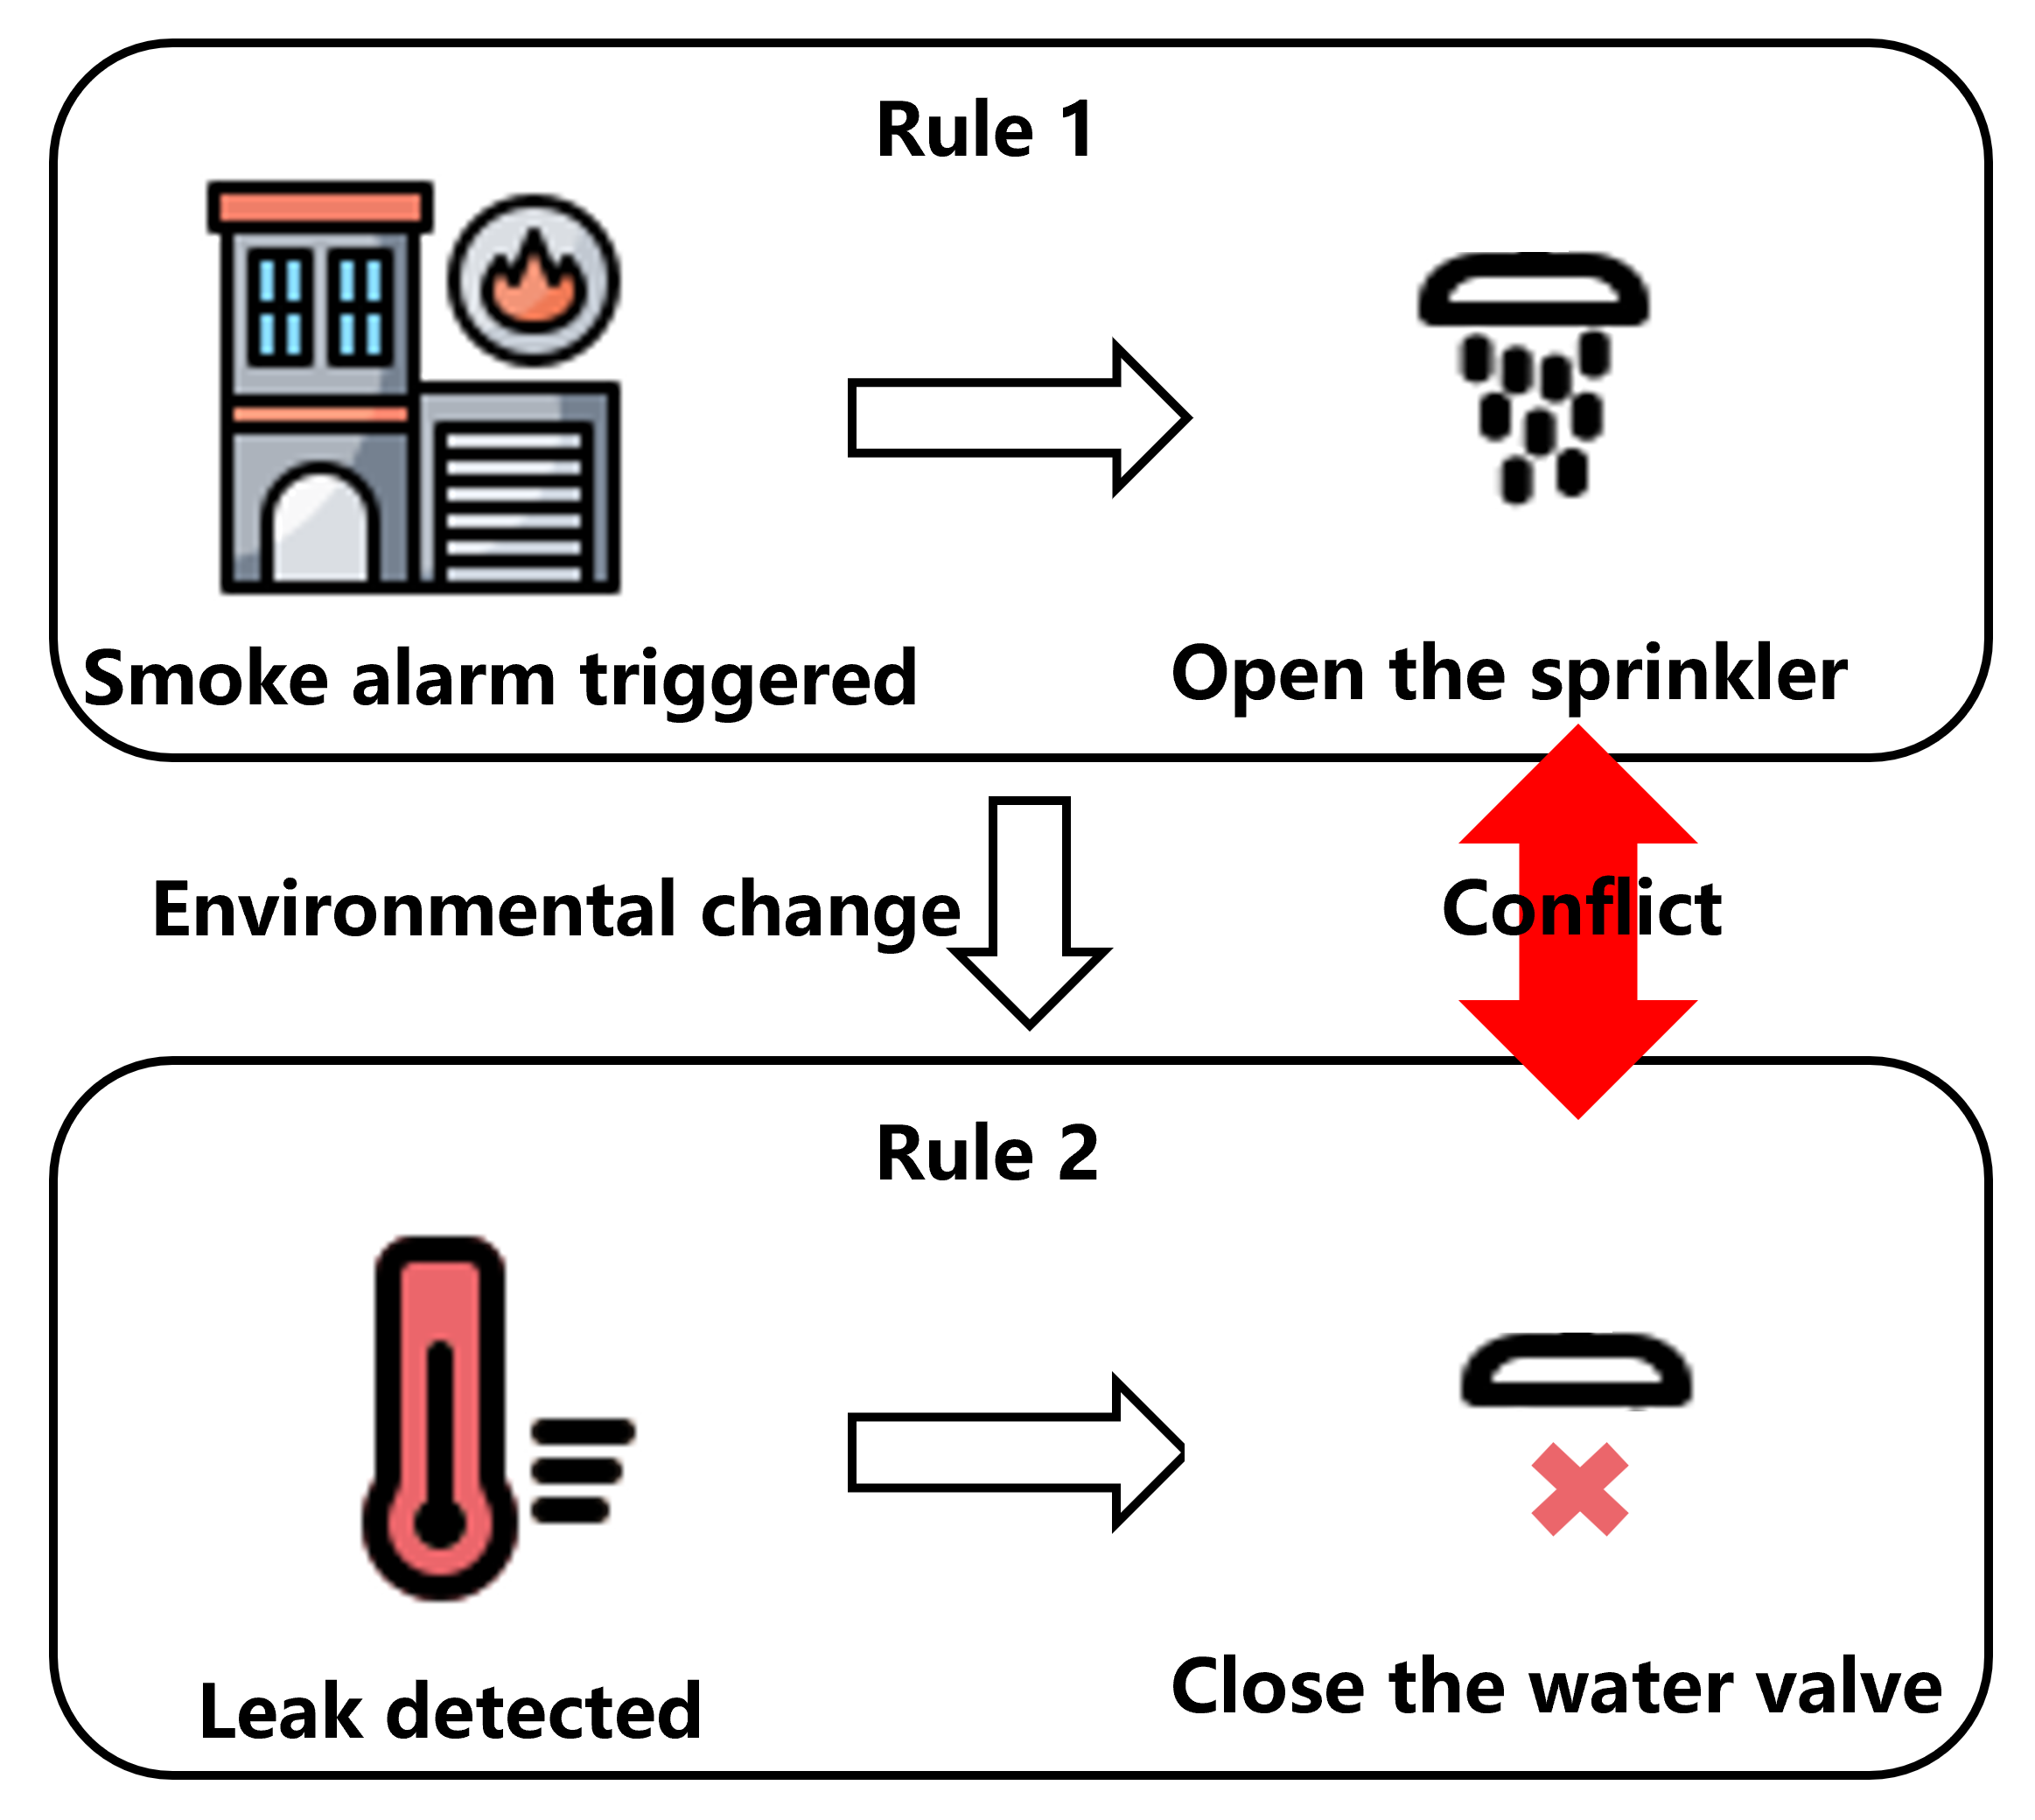
\includegraphics[width=0.4\textwidth]{figure/rule_conflict_example.png}
	\caption{Rule Conflict Example}
	\label{rule_conflict_example}
\end{figure}

% 针对智能家居中存在的规则冲突问题,目前已有一些研究致力于此。现有的规则冲突检测方法大致可以分为两类:(1)基于安全策略的方法:预先定义一套安全策略,若检测到当前规则的执行违反了这些策略,则判定为规则冲突;(2)基于规则交互模式的方法:根据规则之间的交互模式进行检测,若满足某种预定义的交互模式,则认为存在规则冲突的风险。
Several studies have addressed the issue of rule conflicts in smart homes\cite{alhanahnah2020scalable,chen2019multi,chi2020cross,ding2021iotsafe,huang2021conflict,li2020diac,xiao2019a3id,nakamura2005feature,igaki2010modeling,ibrhim2020formal,pradeep2021automating,shehata2007using,sun2014conflict,alharithi2019detecting,celik2019iotguard,hamza2022hsas,leelaprute2008detecting,trimananda2020understanding,yagita2015application,yu2022tapinspector,chaki2020fine,chi2023detecting,celik2018soteria,alhanahnah2022iotcom,ding2018safety,hsu2019safechain,wang2019charting}. Existing rule conflict detection methods can be broadly categorized into two types: (1) Security policy-based methods: A set of security policies is pre-defined, and any rule execution that violates these policies is flagged as a conflict\cite{celik2018soteria,celik2019iotguard,ding2021iotsafe}. (2) Rule interaction pattern-based methods: Detection is based on the interaction patterns between rules, and if a pre-defined interaction pattern is matched, a potential rule conflict is identified\cite{chi2020cross,chi2023detecting,celik2019iotguard,alhanahnah2022iotcom}.

% 规则冲突的处理方法主要有以下三种:(1)重新配置规则:修改或调整已有的规则,以消除冲突。(2)设置安全策略:定义特定的安全策略,确保即使发生规则冲突,执行结果也不会违反这些策略。(3)定制处理方法:针对特定的规则冲突,预定义专门的处理策略。这种方法可以看作是安全策略的扩展,为不同的冲突提供更精细化的解决方案。
Rule conflict resolution methods are mainly divided into the following three categories: (1) Rule reconfiguration: Existing rules are modified or adjusted to eliminate conflicts\cite{celik2018soteria,chen2019multi,chi2020cross,ding2018safety,hsu2019safechain,wang2019charting}. (2) Security policy enforcement\cite{celik2019iotguard,ding2021iotsafe}: Specific security policies are defined to ensure that execution results do not violate these policies, even if rule conflicts occur. (3) Custom resolution methods\cite{chi2023detecting}: Dedicated resolution strategies are pre-defined for specific rule conflicts. This approach can be viewed as an extension of security policies, providing more fine-grained solutions for different conflicts.

% 虽然现有的规则冲突解决方案在一定程度上缓解了该问题,但仍然存在一些局限性。
While existing rule conflict resolution schemes alleviate the problem to some extent, they still have certain limitations.

% 在规则冲突检测方面存在以下问题
The following issues exist regarding rule conflict detection.
\begin{itemize}
	% \item 依赖预定义的策略进行冲突检测的方法,无法覆盖所有可能的冲突场景。智能家居系统具有高度的个性化,通用的安全策略难以适用于所有家庭。例如,对于“检测到烟雾时开启喷淋”的规则,在某些家庭适用,但在另一些家庭可能不适用(例如,只希望在确认有明火时才开启喷淋)。不完备的安全策略会导致部分规则冲突无法被检测到。
	\item Detection methods\cite{celik2018soteria,celik2019iotguard,ding2021iotsafe} that rely on pre-defined policies for conflict detection cannot cover all possible conflict scenarios. Smart home systems are highly personalized, and generic security policies are difficult to apply to all households. For example, the rule "open the sprinkler when smoke is detected" may be appropriate in some homes, but not in others (e.g., only wanting to open the sprinkler when open flames are confirmed). Incomplete security policies can lead to the failure to detect some rule conflicts.
	
	% \item 基于规则交互模式的检测方法,容易产生误报。规则交互本身并不等同于规则冲突,其有效性高度依赖于具体的应用环境和用户偏好。例如,“日落时开启暖气”和“温度达到30\celsius时打开窗户并关闭暖气”这两条规则,在室内花园中可能是合理的,但在卧室中可能会导致能源浪费或不适。
	\item Detection methods\cite{chi2020cross,chi2023detecting,celik2019iotguard,alhanahnah2022iotcom} based on rule interaction patterns are prone to false positives. Rule interaction itself is not equivalent to a rule conflict, and its validity is highly dependent on the specific application environment and user preferences. For example, the rules "turn on the heating at sunset" and "open the window and turn off the heating when the temperature reaches 30\celsius" may be reasonable in an indoor garden, but could lead to energy waste or discomfort in a bedroom.
\end{itemize}

% 在规则冲突处理方面存在以下问题:
The following issues exist regarding rule conflict resolution.
\begin{itemize}
	% \item 直接修改规则配置可能会导致规则失效或引入新的冲突。简单地修改现有规则并不能保证完全解决问题,反而可能带来新的问题。
	\item Directly modifying rule configurations may cause the rules to malfunction or introduce new conflicts. Simply modifying existing rules does not guarantee a complete solution and may introduce new problems\cite{celik2018soteria,chen2019multi,chi2020cross,ding2018safety,hsu2019safechain,wang2019charting}.
	
	% \item  采用通用的安全策略,虽然可以在一定程度上保障家居安全,但缺乏个性化,无法满足不同用户的需求。
	\item While enforcing generic security policies can provide a certain level of home security, they lack personalization and cannot meet the needs of different users\cite{celik2019iotguard,ding2021iotsafe}.
\end{itemize}

\begin{figure}[htbp]
	\centering
	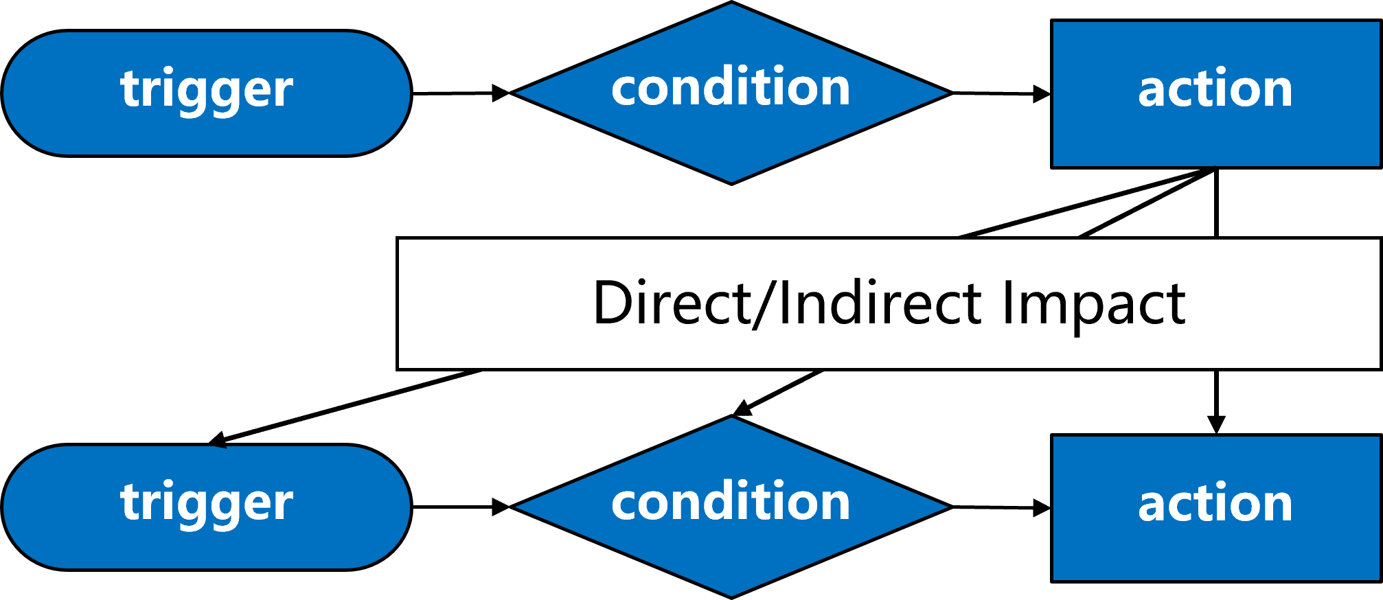
\includegraphics[width=0.4\textwidth]{figure/classification_observation.png}
	\caption{Rule Interaction Pattern}
	\label{classification_observation}
\end{figure}

% 为了解决这些问题,本研究基于以下观察:(1)规则可以使用TCA表示,一条规则可能对另一条规则的触发器、条件和动作产生直接或者间接影响,因此规则之间的交互可以归纳为六种类型 (如图 \ref{classification_observation}所示):一条规则的执行结果可能直接或间接地影响另一条规则的触发、条件或动作。(2)规则交互是否构成冲突是主观的,取决于用户的偏好。(3)智能家居系统通常采用TCA模型来执行规则,但是在规则冲突的检测与处理中还需要考虑到其他通道的影响,且具有区域特征,例如开放式厨房的布局下厨房的温度与湿度特征可能与客厅的温度与湿度特征相关联,而与卧室的温度与湿度特征往往不相关,因此需要对规则特征进行更多的信息采样。
To address these issues, this study is based on the following observations: (1) Rules can be represented using the TCA model, where one rule may directly or indirectly affect the trigger, condition, and action of another rule. Therefore, interactions between rules can be categorized into six types (as shown in \ref{classification_observation}): the execution result of one rule may directly or indirectly affect the trigger, condition, or action of another rule. (2) Whether rule interactions constitute conflicts is subjective and depends on user preferences. (3) Smart home systems typically use the TCA model to execute rules, but the detection and handling of rule conflicts require considering the influence of other channels and have regional characteristics. For example, in an open kitchen layout, the temperature and humidity characteristics of the kitchen may be related to those of the living room, but often unrelated to those of the bedroom. Therefore, more information sampling of rule features is needed.

% 基于以上观察,本文提出了一种新的规则冲突检测与解决方法。首先,我们基于规则交互模式对交互类型进行分类。为了捕获间接通道的影响,本研究通过结合用户环境配置来对规则重新建模,并使用形式化分析方法进行模型检查,以发现所有可能的规则交互。然后,我们结合实体的用户安全配置来实现基本的冲突检测和冲突解决方法策略建议。用户也可以根据自己的偏好进行调整。此外,本研究充分利用了智能家居系统基于TCA模型执行规则的事实,并且当发生规则冲突时,可以选择性地执行规则,从而为每对冲突规则实现定制化的解决方法策略,而不是采用一刀切的通用安全策略。
Based on the above observations, this paper proposes a new rule conflict detection and resolution method. First, we classify interaction types based on rule interaction patterns. To capture the impact of indirect channels, this study re-models rules by incorporating user environment configurations and uses formal analysis methods for model checking to discover all possible rule interactions. Then, we combine the user's security configurations for entities to implement basic conflict detection and conflict resolution strategy recommendations. Users can also make adjustments according to their own preferences. Furthermore, this study takes full advantage of the fact that smart home systems execute rules based on the TCA model, and when rule conflicts occur, rules can be selectively executed, thereby enabling customized resolution strategies for each pair of conflicting rules, rather than adopting a one-size-fits-all general security policy.

% 总而言之,我们的贡献如下:
In summary, we make the following contributions:

\begin{itemize}
	% \item 我们提出了一种基于规则执行机制的规则冲突分类方法,该方法涵盖了所有规则交互类型。
	\item We propose a rule conflict classification method based on the rule execution mechanism that covers all rule interaction types.
	
	% \item 我们设计并实现了一种结合静态和动态冲突检测的方案,适用于智能家居规则的广泛冲突检测机制:通过为规则增加区域属性并重新建模,结合安全实体配置进行静态冲突检测;同时,采用断言检测的方法在运行时检测系统中是否存在规则冲突。
	\item We design and implement a solution combining static and dynamic conflict detection to achieve a widely applicable conflict detection mechanism suitable for smart home rules: Static conflict detection is performed by adding region attributes to the rules and remodeling them, combined with security entity configuration; at the same time, assertion detection methods are used to detect whether rule conflicts exist in the system during runtime.
	
	% \item 我们设计并实现了冲突解决方案、定制化的冲突规则处理策略以及冲突预防措施:基于规则执行机制,实现了多种冲突处理策略,并根据安全实体配置自动选择合适的处理策略。此外,还可以在规则冲突发生前进行拦截,以防止冲突发生。
	\item We design and implement conflict resolution solutions, customized conflict rule resolution strategies, and conflict prevention measures: Based on the rule execution mechanism, multiple conflict resolution strategies have been implemented, and appropriate resolution strategies are automatically selected based on security entity configuration. In addition, conflicts can be intercepted before they occur to prevent conflicts from occurring.
\end{itemize}

\section{Motivated Example}

\begin{figure}[htbp]
	\centering
	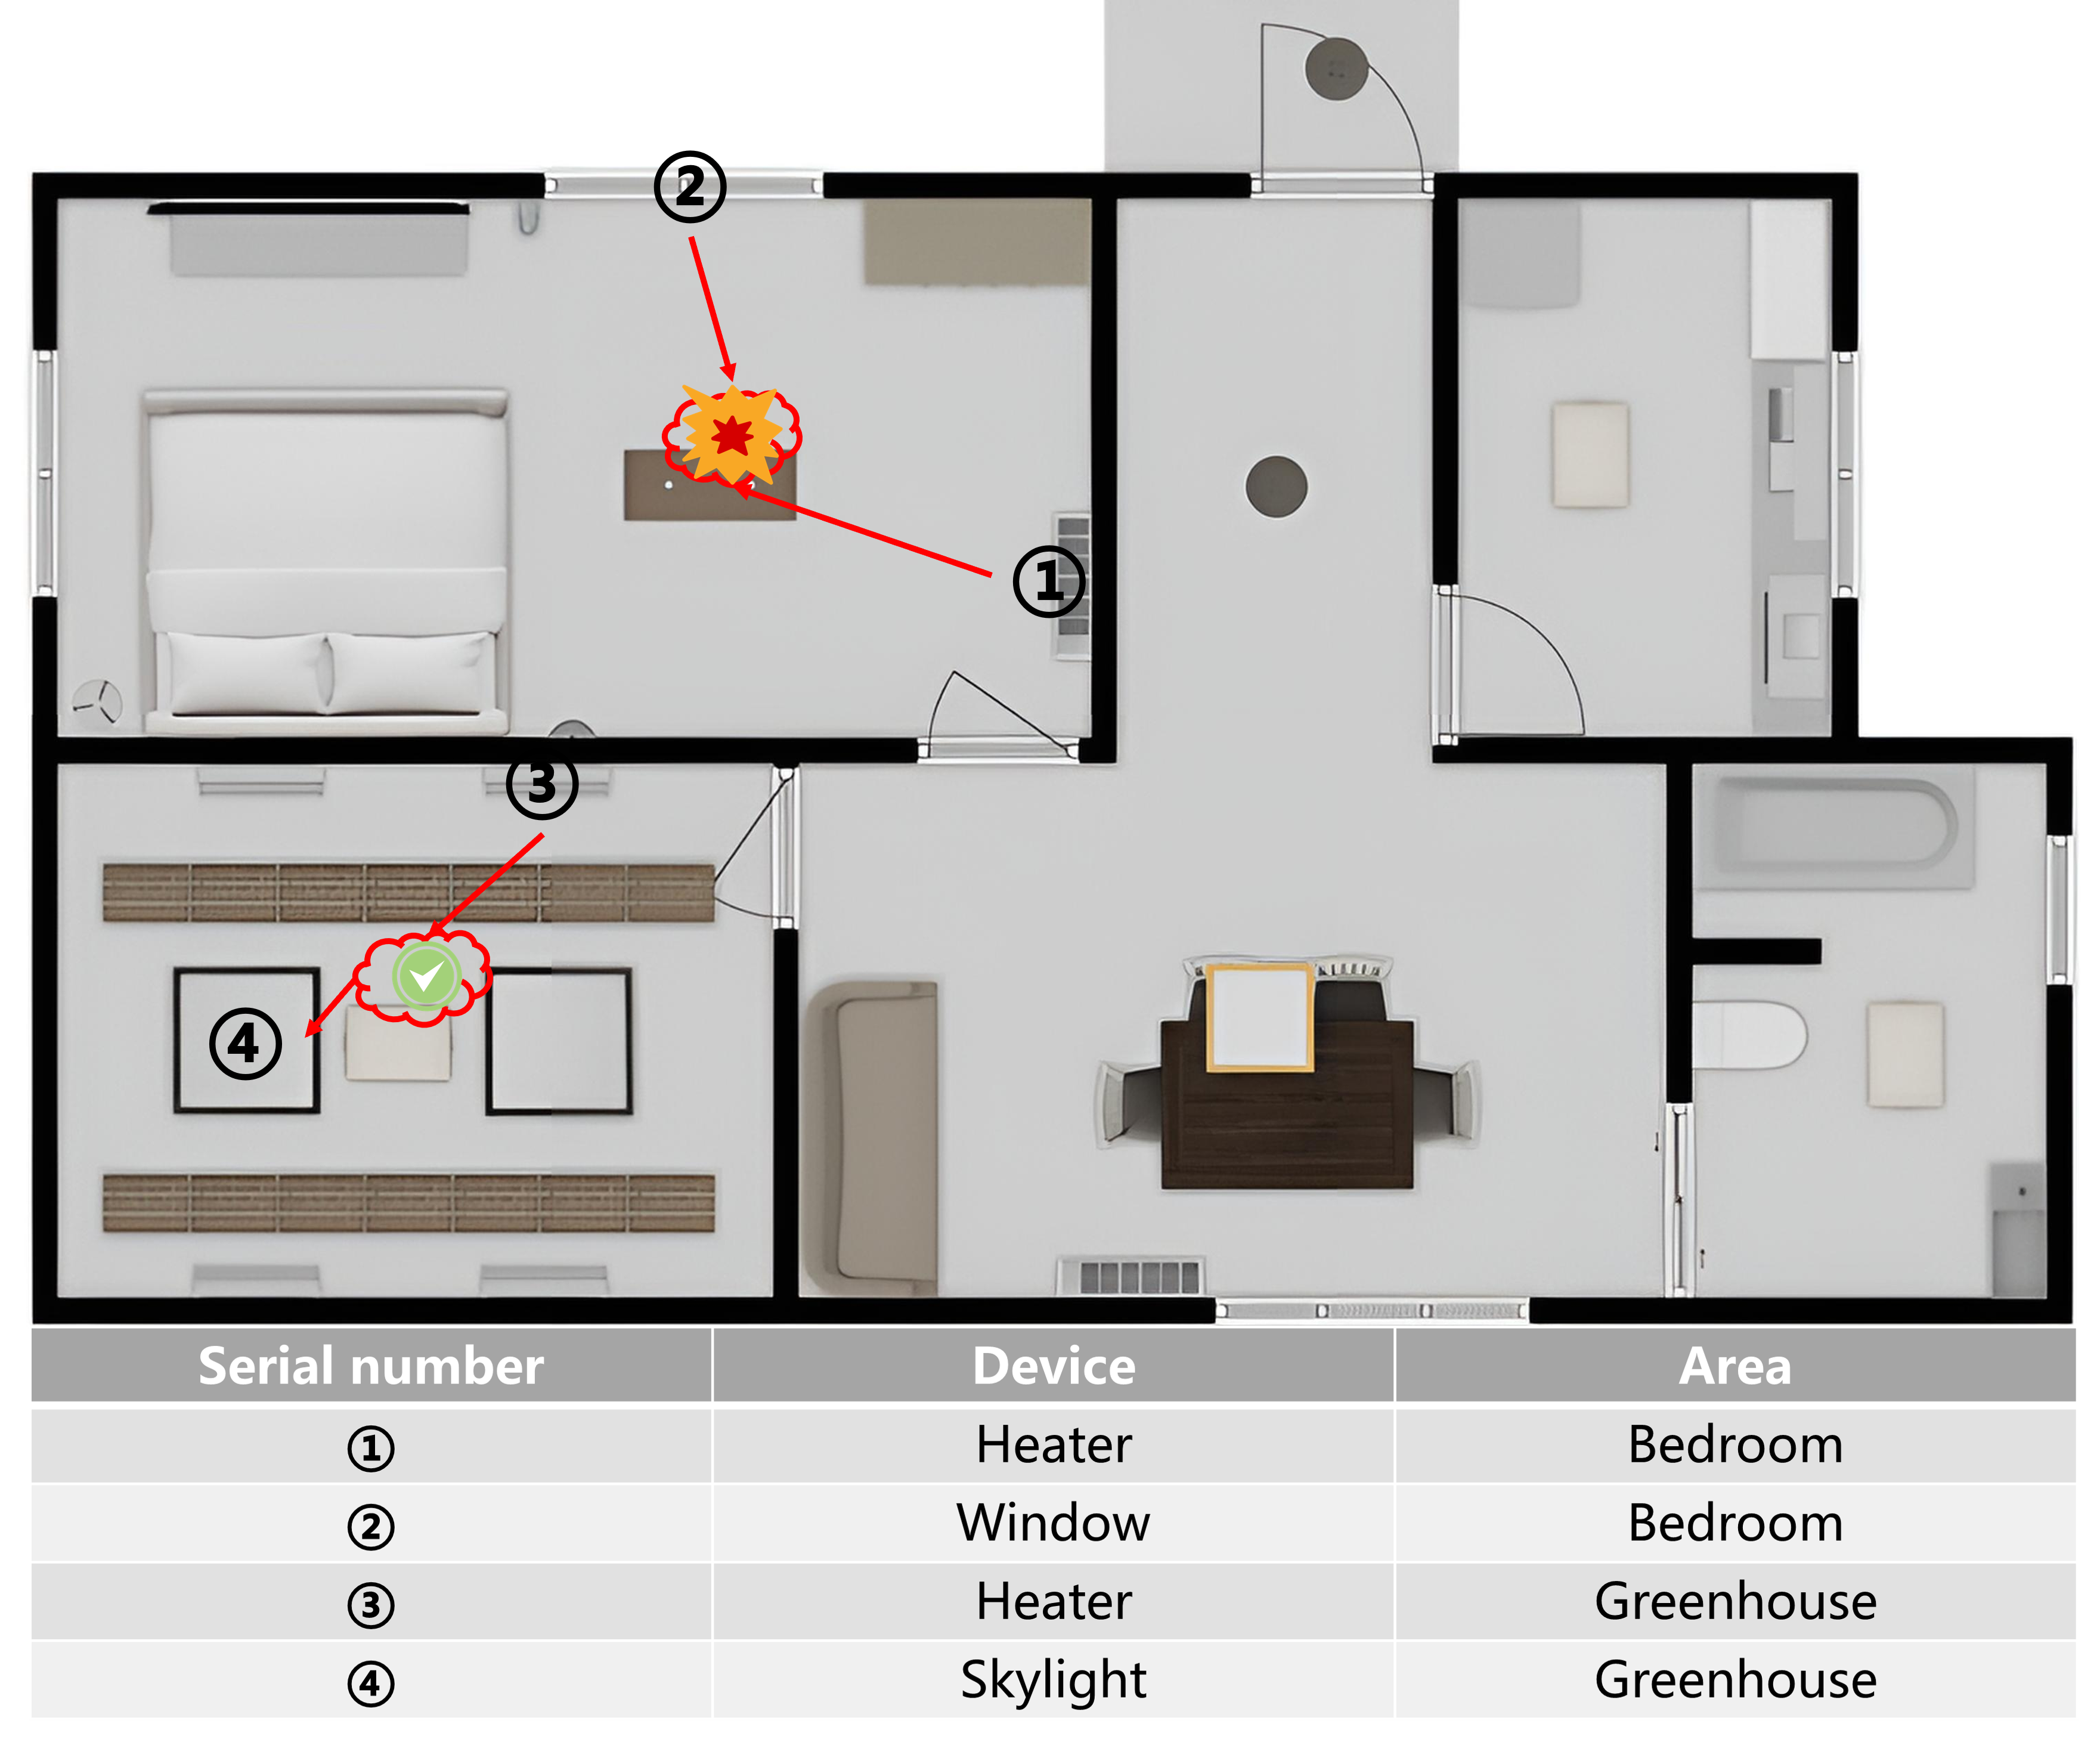
\includegraphics[width=0.4\textwidth]{figure/motivated_example.png}
	\caption{Motivated Example}
	\label{motivated_example}
\end{figure}

%这一章节将使用具体实例来展示规则冲突的一些性质以及当前规则冲突检测与环节方法存在的缺陷。Fig.\ref{smarthome_floorplan}展示了一个智能家居平面图,共包括Outdoor(中间上方)、porch(中间)、living room(中间下侧)、 kitchen(中间右侧)、batch room(右下侧)、 bedroom(中间左侧)和green house(garden,左下侧)7个区域。
In this section, specific examples will be used to demonstrate some properties of rule conflicts, as well as the shortcomings of current rule conflict detection and mitigation methods. Fig. \ref{motivated_example} shows a smart home floor plan, including seven areas: Outdoor (top center), porch (center), living room (bottom center), kitchen (bottom right), batch room (bottom right), bedroom (center left), and green house (garden, bottom left).

%在green house中设定自动化规则1,触发条件为\texttt{日落},执行动作是\texttt{打开加热器}。同时设定自动化规则2,触发条件为\texttt{温度达到三十摄氏度},执行动作是\texttt{打开窗户并关闭加热器}。如Fig.\ref{motivated_example}中左下角展示的那样,当日落时在green house中首先自动执行了规则1,加热器打开为green house持续供暖,温度持续上升可能超过30摄氏度,此时自动化规则1的执行结果通过影响室内温度从而触发自动化规则2的执行,使得加热器关闭并且打开天窗。在green house中打开天窗往往是符合用户预期且安全的,但是如果这两条规则设置在用户的卧室中,则情况会明显不同:规则1通过提高卧室温度触发规则2的执行,打开,了卧室的窗户,卧室的窗户往往不是天窗,而且如果在用户预期之外打开卧室窗户则会给智能家居系统引入安全隐患,甚至被攻击者恶意利用规则从而创造规则执行的通路来控制窗户、门锁等安全敏感设备。
In the greenhouse, automation rule 1 is set with the trigger condition being \texttt{sunset}, and the action is \texttt{turn on the heater}. Simultaneously, automation rule 2 is set with the trigger condition being \texttt{temperature reaches thirty degrees Celsius}, and the action is \texttt{open the windows and turn off the heater}. As shown in the bottom left corner of Fig.\ref{motivated_example}, when the sun sets in the greenhouse, rule 1 is automatically executed first, and the heater is turned on to continuously provide heat to the greenhouse. The temperature may continue to rise above 30 degrees Celsius. At this time, the execution result of automation rule 1 affects the indoor temperature, thereby triggering the execution of automation rule 2, which turns off the heater and opens the skylight. Opening the skylight in the greenhouse is often in line with user expectations and is safe. However, if these two rules are set in the user's bedroom, the situation will be significantly different: rule 1 triggers the execution of rule 2 by raising the bedroom temperature, opening the windows of the bedroom. The windows of the bedroom are often not skylights, and opening the bedroom windows unexpectedly can introduce security risks to the smart home system, and attackers may even maliciously use the rules to create execution paths to control security-sensitive devices such as windows and door locks.

%以上示例表明,规则交互可能并非由一条规则的执行动作直接影响另一条规则(例如两条同时执行的规则,一个控制空调为加热模式,一个控制空调为制冷模式),也可能通过间接通道产生交互(常见的有温度、湿度、亮度、声音等等),在检测规则冲突时需要考虑到源于其它通道的规则冲突。同时还能观察到规则冲突具有区域性和用户的主观性。以上规则交互如果发生在green house就不被视为规则冲突,发生在卧室则可能被视为规则冲突,用户的主观性体现在针对一对规则交互,有的用户可能将其视为规则冲突,有的用户认为是正常的规则交互(例如卧室空调的除湿模式和加湿器交替工作维持空气湿度保持在适宜的水平,有的用户认为是正常交互,还有用户可能会认为是浪费资源)。除此之外,上述示例还能表明在智能家居系统中对侧面通道的检测不能仅仅通过温度、湿度等参数界定,还应该具有区域属性,例如porch的灯光可能影响到厨房和客厅的亮度、却并不会影响到卧室的亮度,如果两个与亮度相关的规则同时执行可能并不会发生交互。
The above examples show that rule interactions may not be directly influenced by the execution action of one rule on another (e.g., two rules executing simultaneously, one controlling the air conditioner to heat mode and the other to cool mode), but may also be generated through indirect channels (commonly temperature, humidity, brightness, sound, etc.). When detecting rule conflicts, it is necessary to consider rule conflicts originating from other channels. At the same time, it can be observed that rule conflicts have regionality and user subjectivity. The above rule interaction may not be regarded as a rule conflict if it occurs in a greenhouse, but it may be regarded as a rule conflict if it occurs in a bedroom. User subjectivity is reflected in the fact that for a pair of rule interactions, some users may regard it as a rule conflict, while others may regard it as a normal rule interaction (for example, the dehumidification mode of the bedroom air conditioner and the humidifier work alternately to maintain the air humidity at a suitable level, some users think it is a normal interaction, while others may think it is a waste of resources). In addition, the above examples also show that the detection of side channels in smart home systems should not be limited to temperature, humidity and other parameters, but should also have regional attributes. For example, the porch lights may affect the brightness of the kitchen and living room, but will not affect the brightness of the bedroom. If two brightness-related rules are executed at the same time, they may not interact with each other.

%针对以上示例,如果采用特定的安全策略的方法进行检测需要用户付出大量的effort,因为不同家庭因为户型、设备等差异性导致不同的家庭都需要相关专业人员设定所有安全策略,且安全策略很可能包含所有的规则冲突。如果根据自动化规则交互模式进行判断,确实能够检测到卧室中发生的规则冲突,但是也会将green house中的规则交互视为规则冲突,当设定的自动化规则数量增多,容易产生大量的误报需要用户逐个确认,也会导致较大的user's effort。
It requires a lot of effort for users to set all security policies using specific security strategies to detect potential risks, because different families need relevant professionals to set all security policies due to differences in housing types, equipment, etc., and security policies are likely to contain all rule conflicts. If the judgment is made based on the automatic rule interaction mode, the rule conflict that occurs in the bedroom can indeed be detected, but the rule interaction in the green house will also be regarded as a rule conflict. When the number of set automatic rules increases, a large number of false positives are likely to occur and need to be confirmed by users one by one, which will also lead to a large user's effort.
\section{Design}

\subsection{Overview}
\begin{figure*}[htbp]
	\centering
	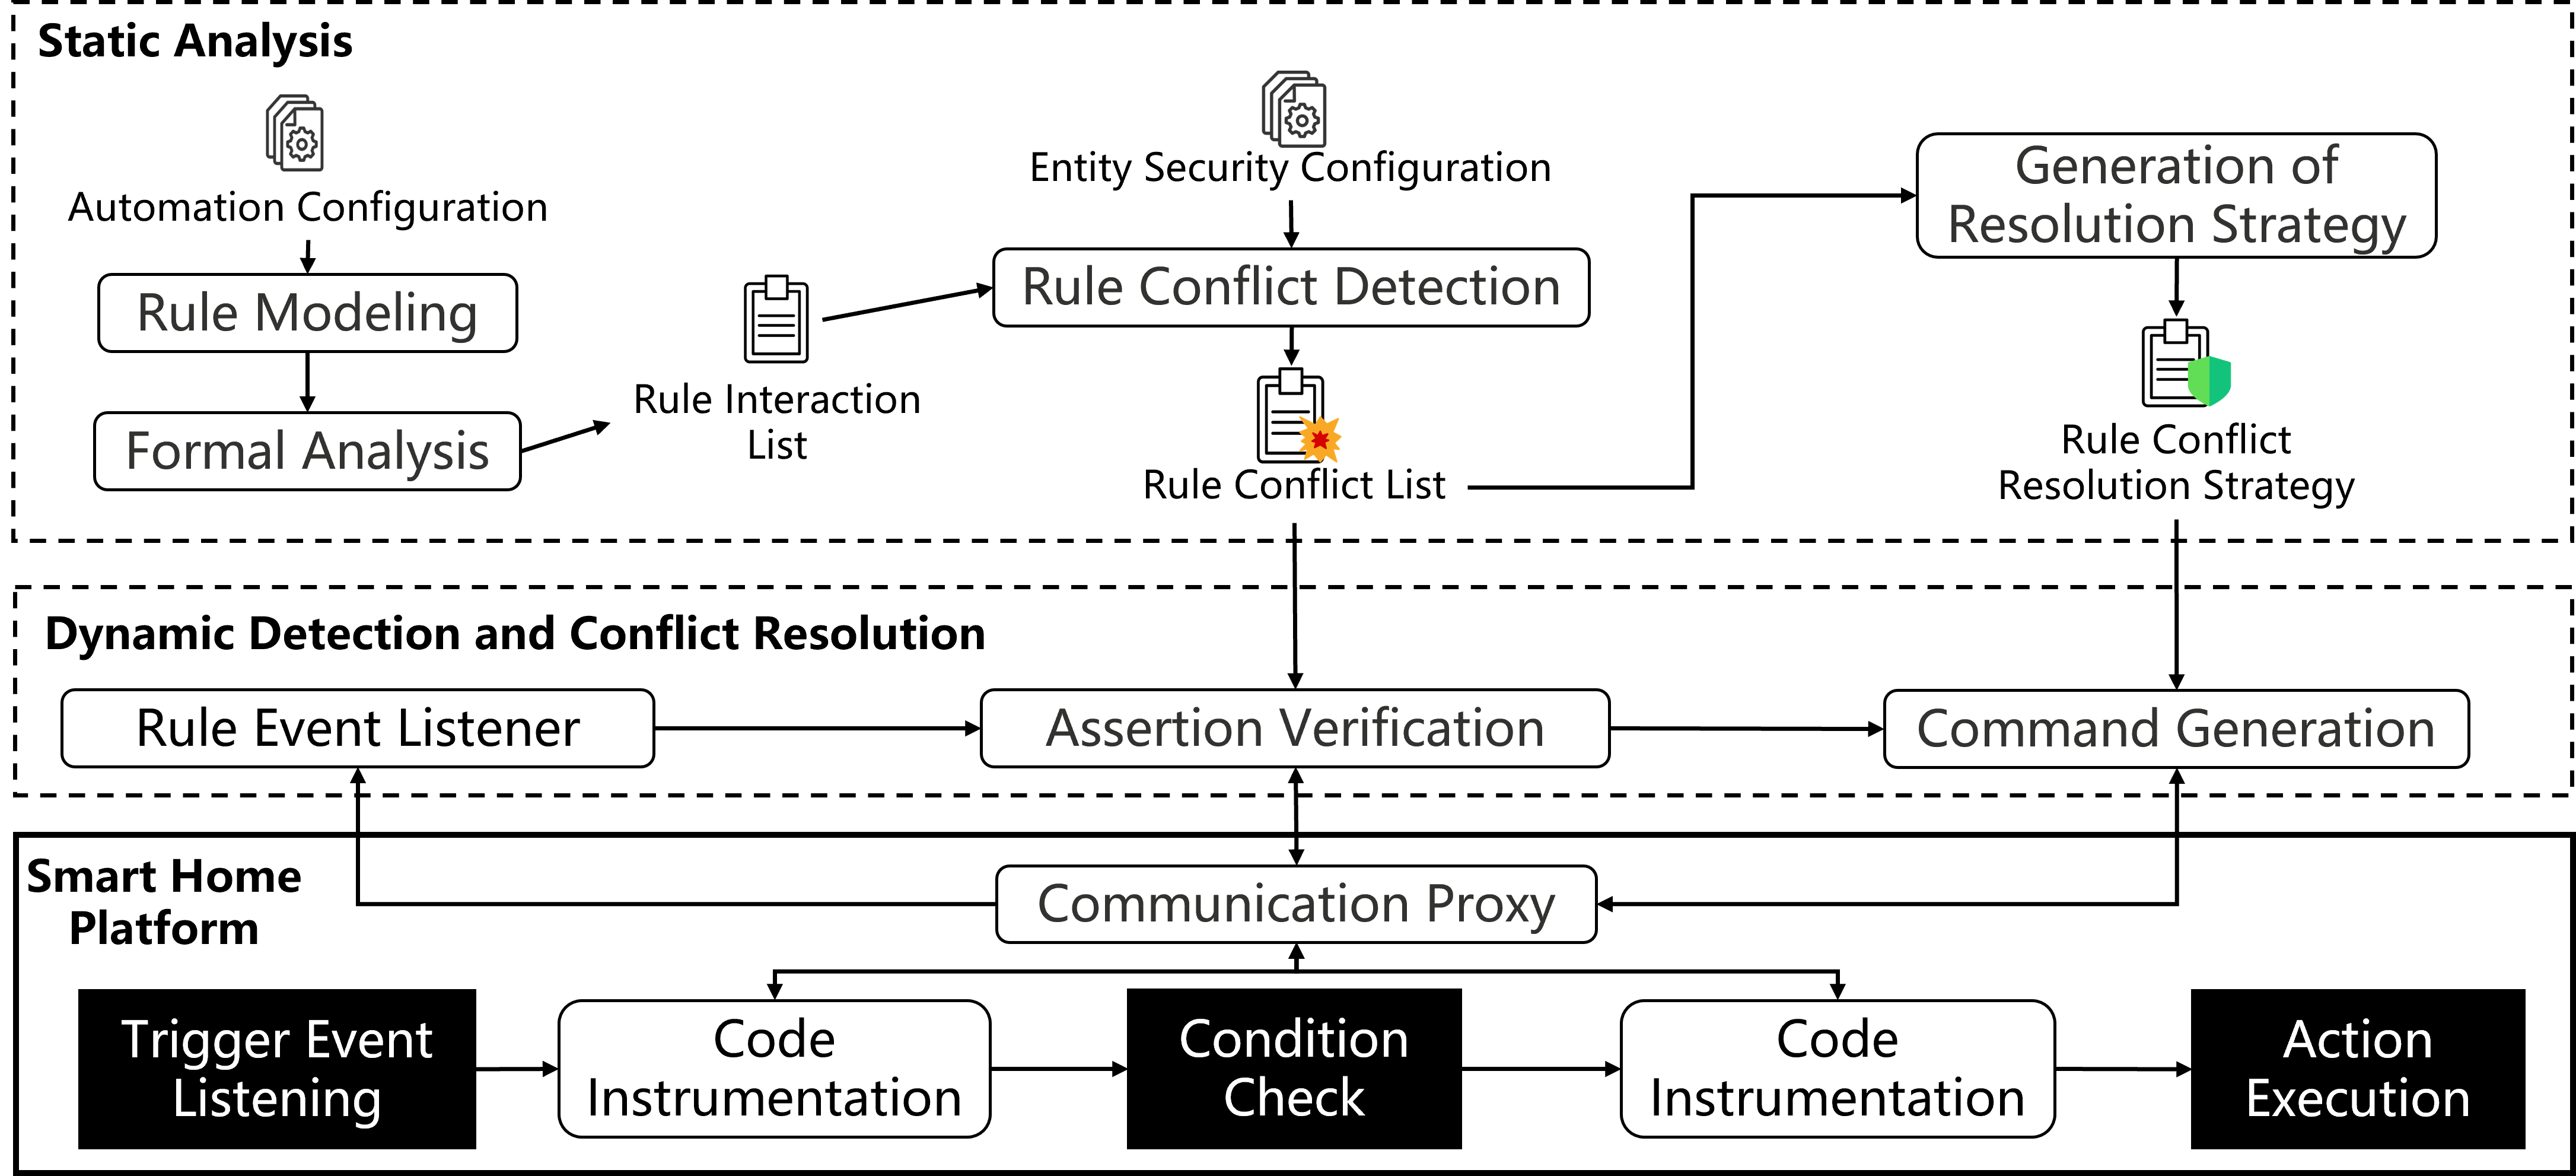
\includegraphics[width=\textwidth]{figure/overall_design.png}
	\caption{Overall Architecture of Our Approach}
	\label{overall_design}
\end{figure*}
% 本文设计了一个完整的系统,旨在通过静态与动态分析相结合的方式检测规则交互中存在的潜在规则冲突,并在冲突发生前自动执行定制化的冲突处理策略,避免实际冲突的发生。如图 Fig.\ref{overall_design} 所示,我们的方法主要包括两个阶段:1) 静态分析;2) 动态检测与冲突处理。
This paper presents a complete system designed to detect potential rule conflicts within rule interactions through a combination of static and dynamic analysis. The system automatically executes customized conflict resolution strategies before conflicts occur, preventing their actual manifestation. As illustrated in Fig.\ref{overall_design}, our approach primarily comprises two phases: 1) Static Analysis; 2) Dynamic Detection and Conflict Resolution.

% 静态分析阶段包含规则建模模块、形式化分析模块、静态规则冲突检测模块以及冲突处理策略生成模块。首先,对智能家居系统中的规则进行重新建模,以区分家庭环境中的不同区域。然后,形式化分析模块基于新的规则模型提取所有类型的规则交互,并生成相应的交互分析数据。用户的实体安全配置将应用于静态规则冲突检测模块,用于从规则交互集合中识别出真正的规则冲突。考虑到规则交互是否构成冲突具有主观性,系统提供用户配置界面,以自然语言的形式展示形式化分析模块提取的规则交互分析数据,辅助用户进行冲突判定。最后,冲突处理策略生成模块为每个已识别的规则冲突生成定制化的处理策略。
The static analysis phase includes a rule modeling module, a formal analysis module, a static rule conflict detection module, and a conflict resolution strategy generation module. Initially, the rules in the smart home system are remodeled to differentiate between zones within the environment. Subsequently, the formal analysis module extracts all types of rule interactions based on the new rule model and generates corresponding interaction analysis data. The user's entity safety configuration is then applied to the static rule conflict detection module, which identifies actual rule conflicts from the set of rule interactions. Recognizing the subjectivity inherent in defining a rule interaction as a conflict, the system presents the rule interaction data extracted by the formal analysis module to the user through a user configuration interface in natural language in order to facilitate the user determining rule conflicts. Finally, the conflict resolution strategy generation module generates customized resolution strategies for each identified rule conflict.

% 动态检测与冲突处理阶段包含规则事件监听模块、断言验证模块和命令生成模块。此外,智能家居系统(例如 Home Assistant)中的代码插桩模块将辅助完成动态规则冲突检测与预防。规则事件监听模块实时监听规则执行信息。当一条规则被触发,并在条件检查前后,该模块会将相关信息发送给断言验证模块。断言验证模块将基于历史规则执行事件、当前执行规则信息以及相关设备状态信息进行断言验证,判断规则冲突是否实际发生。若确认冲突即将发生,命令生成模块将根据静态分析阶段生成的冲突处理策略,生成相应的执行命令,并由代码插桩模块强制执行。
The dynamic detection and conflict resolution phase includes a rule event listener module, an assertion verification module, and a command generation module. Additionally, the code instrumentation module within the smart home system (e.g., Home Assistant) assists in dynamic rule conflict detection and prevention. The rule event listener module monitors the rule execution information in real time. When a rule is triggered, the listener module sends related information to the assertion verification module both before and after condition checking. Based on historical rule execution events, current rule information, and relevant device state information, the assertion verification module then performs assertion verification to determine whether a rule conflict has indeed occurred. If so, the command generation module will generate execution commands with the current rule conflict information about to occur and the rule conflict resolution strategy from static detection, which will be enforced by the code instrumentation module.

\subsection{Static Analysis}

\subsubsection{Rule Modeling}

%\begin{figure}[htbp]
%	\centering
%	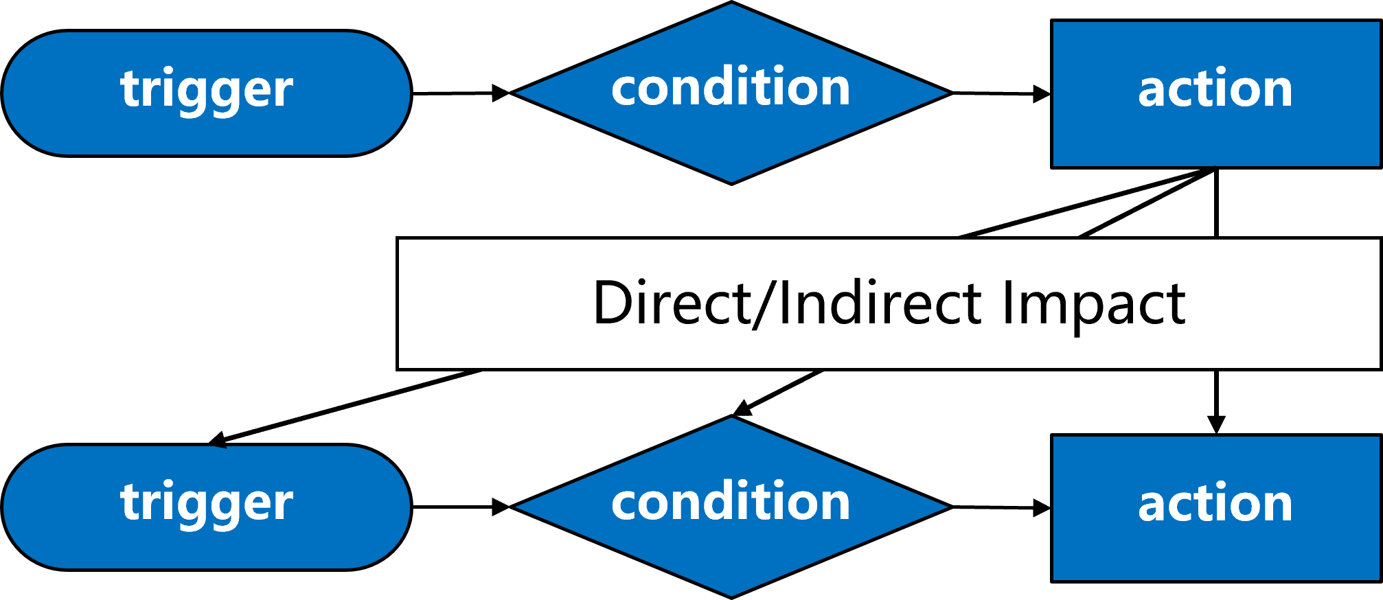
\includegraphics[width=0.4\textwidth]{figure/classification_observation.png}
%	\caption{Rule Interaction Pattern}
%	\label{classification_observation}
%\end{figure}

% 在介绍静态阶段之前,首先阐述本方案对规则交互与规则冲突的分类方法。基于之前的观察,我们将规则之间的交互归纳为:一条规则的执行结果对另一条规则的触发器、条件或动作产生直接或间接的影响。由此,我们将规则交互分为以下几类:触发器交互 (Trigger Interaction)、条件交互 (Condition Interaction)、动作交互 (Action Interaction)、间接触发器交互 (Indirect Trigger Interaction)、间接条件交互 (Indirect Condition Interaction) 和间接动作交互 (Indirect Action Interaction)。相应地,我们定义了六种规则冲突类型:触发器冲突 (Trigger Conflict)、条件冲突 (Condition Conflict)、动作冲突 (Action Conflict)、间接触发器冲突 (Indirect Trigger Conflict)、间接条件冲突 (Indirect Condition Conflict) 和间接动作冲突 (Indirect Action Conflict)。
Before formally introducing the static phase, it is necessary to the classification of rule interactions and rule conflicts for this approach. Based on previous observations Fig.\ref{classification_observation}, we summarize the interactions among rules as follows: the execution result of one rule can have direct and indirect impacts on the triggers, conditions, and actions of another rule. Thus, we can classify rule interactions as follows: Trigger Interaction, Condition Interaction, Action Interaction, Indirect Trigger Interaction, Indirect Condition Interaction, and Indirect Action Interaction. At the same time, six categories of rule conflicts can be identified: Trigger Conflict, Condition Conflict, Action Conflict, Indirect Trigger Conflict, Indirect Condition Conflict, and Indirect Action Conflict.

% 智能家居系统中的规则通常以静态文件形式存储,从中可以提取规则的触发器 (T)、条件 (C) 和动作 (A) 属性,并快速建模为 $\langle T,C,A \rangle$ 模型。然而,仅凭这些数据不足以检测不同家庭区域中侧面通道的影响,例如不同规则对卧室温度的影响所引发的交互,或者不同规则开启高功耗设备导致家庭用电功率升高,从而触发节电规则等。因此,需要引入新的属性 $E$。定义 $E=[e^1, e^2,\dots]$,$e^i=(area, channel, trend)$。其中,$area$ 表示间接通道的区域特征,如厨房、客厅或整个家庭等;$channel$ 表示侧面通道名称,如温度、湿度、光照强度等;$trend$ 表示该侧面影响的影响趋势,如升高、降低等。对于规则的触发器或条件,如果 $e$ 为 $\langle kitchen, temperature, increases\rangle$,则表示其他规则的执行结果可能导致厨房温度升高,从而使当前规则的触发器更易触发或条件更易满足。对于规则的动作,如果 $e$ 为 $\langle kitchen, temperature, increases\rangle$,则表示当前规则的执行可能导致厨房温度升高。属性 $E$ 基于用户真实的家庭情况和相关规则确定。例如,如果一个家庭中没有任何与 "湿度" 相关的规则,则无需将 $channel$ 设置为 "湿度"。由此,规则可以被重新建模为 $R=\langle T,C,A,E\rangle $ 或 $R=\langle T,C,A,E_T,E_C,E_A \rangle$ 形式,称为 TCAE 模型。
In smart home systems, rule configuration is usually stored as static files, from which the triggers, conditions, and action attributes of a rule can be extracted, and quickly modeled as a $\langle T,C,A \rangle$ model. However, the above data is insufficient to support the detection of the effects of side channels in different home areas within smart home systems. For example, rule interactions may be caused by different rules affecting the bedroom temperature, or by different rules turning on high-power devices, leading to an increase in the household's power consumption and subsequently triggering related rules to conserve electricity. Therefore, a new attribute $E$ needs to be introduced. $E$ is defined as$E=[e^1, e^2,\dots]$ and $e^i=(area, channel, trend)$, where $area$ indicates the spatial characteristics of the channel, such as the kitchen, living room, or the whole home; $channel$ indicates the name of the other channel which rules may impact each other, such as temperature, humidity, illuminance and so on; and $trend$ indicates the direction of the influence of the other channel, such as an increase and decrease. For the trigger/condition of a rule, if $e$ is $\langle kitchen, temperature, increases\rangle$, it means that if the execution results of other rules may lead to an increase in kitchen temperature, then the trigger/condition of the current rule is more likely to be met. For the action execution of a rule, if $e$ is $\langle kitchen, temperature, increases\rangle$, it means that the execution of the current rule may promote an increase in kitchen temperature. The attribute $E$ will be determined based on the user's actual home situation and the related rules. For example, if there are no rules concerning "humidity" in a home, then there is no need to set the $channel$ attribute of $e$ as "humidity". Thus, a rule can be re-modeled in the following form: $R=\langle T,C,A,E\rangle $ or $R=\langle T,C,A,E_T,E_C,E_A \rangle$ which called TCAE model.

\subsubsection{Formal Analysis}

\begin{table*}[htbp]
	\begin{center}
		\caption{Formal Analysis Expression}
		\label{Formal_Analysis_Expression}
		\begin{adjustbox}{width=0.95\textwidth}
			\begin{tabular}[width=0.95\textwidth]{c|c} 
				\hline
				\textbf{Classification} & \textbf{Expression}\\
				\hline
				\text{Trigger Interaction} & $(\exists a_{1}\in A_{1})\wedge(a_{1}\rightarrow T_{2})$ \\
				\hline
				\text{Condition Interaction} & $\left((A_{1}\nrightarrow C_{2})\wedge\left((T_{1}\neq T_{2})\wedge(R_{1}\neq R_{2})\right)\right)\vee\left((A_{1}\to\mathcal{C}_{2})\wedge\left((T_{1}\neq T_{2})\wedge(R_{1}\neq R_{2})\right)\right)$ \\
				\hline
				\text{Action Interaction} & $(\exists a_{1}\in A_{1})\wedge(\exists a_{2}\in A_{2})\wedge(a_{1}\perp a_{2})$ \\
				\hline
				\text{Indirect Trigger Interaction} & $(\exists a_{1}\in A_{1})\wedge\left(E_{a_{1}}=E_{T_{1}}\right)$ \\
				\hline
				\text{Indirect Condition Interaction} & $\left(\left(E_{A_{1}}\perp E_{C_{2}}\right)\vee\left(E_{A_{1}}=E_{C_{2}}\right)\right)\wedge\left(R_{1}\neq R_{2}\right)$ \\
				\hline
				\text{Indirect Action Interaction} & $(\exists a_{1}\in A_{1})\wedge(\exists a_{2}\in A_{2})\wedge\left(D_{a_{1}}\neq D_{a_{2}}\right)\wedge\left(E_{a_{1}}\perp E_{a_{2}}\right)$ \\
				\hline
			\end{tabular}
		\end{adjustbox}
	\end{center}
\end{table*}

% 基于 TCA 模型进行规则冲突分类,假设规则 $R_1=\langle T_1,C_1,A_1,E_{T_1},E_{C_1},E_{A_1} \rangle$ 和 𝑅₂=(𝑇₂, 𝐶₂, 𝐴₂, 𝐸(𝑇₂), 𝐸(𝐶₂), 𝐸(𝐴₂)) 表示在同一系统中设置的两条规则。其中,T、C、A 和 E 分别表示对应的属性。本文使用 $\rightarrow$ 表示促使触发器触发或条件满足,$\nrightarrow$ 表示禁止条件满足。对于 channel 属性,$\bot$ 表示两个 channel 属性具有相同的 $area$ 和 $channel$,但 $trend$ 相反(例如,厨房温度升高与厨房温度降低)。此外,$\bot$ 也表示两个动作相互冲突(例如,开启空调与关闭空调)。"=" 表示两个 channel 属性具有相同的 $area$、$channel$ 和 $trend$,或者两个触发器或条件相同。
According to the TCA model for rule conflict classification, let rule $R_1=\langle T_1,C_1,A_1,E_{T_1},E_{C_1},E_{A_1} \rangle$ and rule  $R_2=\langle T_2,C_2,A_2,E_{T_2},E_{C_2},E_{A_2} \rangle$ be to represent two rules set in the same system, where T, C, A, and E respectively represent the corresponding attribute. This paper uses $\rightarrow$ to indicate that a trigger is activated or a condition is met, and $\nrightarrow$ to indicate that a condition is prohibited.$\bot$ denotes that the two channel attributes have the same area and channel but opposite trends (for example, rising kitchen temperature versus falling kitchen temperature), or it indicates that two actions are in conflict (such as turning on the air conditioner versus turning it off), while "=" indicates that the two channel attributes have the same area, channel, and trend, or that there are two identical triggers or conditions.

% 形式化分析模块遍历每个规则模型,并进行表达式验证。若表达式成立,则表示两条规则满足对应的规则交互类型。规则冲突是规则交互的特例,因此,该表达式仅用于筛选存在交互的规则,而要判断规则交互是否构成实际的规则冲突,还需要进一步的检测。具体的表达式如 Table.\ref{Formal_Analysis_Expression} 所示。由此,形式化分析模块能够分析得到具体的规则交互列表,其中包含了所有规则交互及其交互模式信息。
The formal analysis module will traverse each rule model and then expression validation. If an expression is satisfied, it indicates that the two rules meet the corresponding rule interaction classification. Rule conflict is a special case of rule interaction, and that expression can only filter out interacting rules. further detection is required to determine whether a rule interaction constitutes a rule conflict.The formal analysis module can analyze and obtain a specific list of rule interactions, which includes all rule interactions and interaction pattern information.

\subsubsection{Rule Conflict Detection and Resolution Strategy Generation}
% 实体安全配置是安全敏感设备实体的安全状态集合,用于表示智能家居系统中发生冲突时应优先保持的状态。例如,门应保持 "关闭" 状态,消防喷淋头应保持 "开启" 状态。规则冲突检测模块对规则交互列表中的每个元素进行实体安全检查,以确定规则交互是否违反实体安全状态,从而引发潜在的规则冲突。
Entity safety configuration is a set of safety states for a security-sensitive device entity, used to indicate the preferred state to maintain when a conflict occurs in a smart home system—for example, a door should be "closed" and a fire sprinkler should be "on." The rule conflict detection module performs an entity safety on all elements in the rule interaction list to determine whether a rule interaction violates the entity safety state, potentially causing a rule conflict.

% 具体的检查方法如下:对于包含两条规则的规则交互,需要关注交互完成后是否违反实体安全配置的要求。为此,为每条规则设定一个安全值参数 $sf$。若规则的执行结果更符合实体安全状态配置,则 $sf$ 值越高,反之越低。$sf$ 值通过遍历所有实体安全配置,采用线性函数计算。例如,若规则的执行结果是关闭门,这符合实体 "门" 的安全状态 "关闭",则该规则的 $sf$ 值在原有基础上加一,反之则减一。默认值为零。
The specific inspection method is as follows: a rule interaction includes two rules, and attention should be paid to whether the entity safety configuration requirements are violated after this rule interaction is completed. Therefore, each rule sets a safety value parameter, $sf$. If the execution result of a rule is more inclined to meet the entity safety configuration, the $sf$ value is higher; otherwise, it is lower. The specific $sf$ value can be calculated using a linear function by traversing all the entity safety configurations. For example, if the execution result of a rule is closing a door, which is more in line with the entity safety state "closed" for the entity "door", then the rule's $sf$ is increased by one from the original value, Otherwise, it is decreased by one, with the default value being zero.

% 针对不同类型的规则交互,规则冲突的判定方法有所不同:
% \begin{itemize}
	% 	\item 对于触发器交互和间接触发器交互,关注第二条规则的安全值 $sf$ 是否大于零。若小于零,则判定为规则冲突。
	% 	\item 对于条件交互和间接条件交互,若第一个规则禁止了第二个规则的条件,且第二个规则的 $sf$ 大于零,则判定为规则冲突;反之,若第一个规则使得第二个规则的条件得以满足,且第二个规则的 $sf$ 小于零,也判定为规则冲突。这表明前一条规则的影响导致后一条更符合实体安全状态的规则未被执行,或导致后一条与实体安全状态相违背的规则被执行。
	% 	\item 对于动作交互和间接动作交互,若其中包含的两条规则的安全值之一不为零,则判定为规则冲突。需要注意的是,即使两条规则的安全值都大于零,仍可能判定为规则冲突,因为此类交互中的两条规则的执行结果是相互矛盾的,通常只需执行其中一条规则。
	% \end{itemize}
For different rule interactions, the method for determining rule conflicts varies. 
\begin{itemize}
	\item For Trigger Interaction and Indirect Trigger Interaction, the focus is on whether the safety value $sf$ of the second rule is greater than zero; if it is less than zero, then it is determined to be a rule conflict.
	\item For Condition Interaction and Indirect Condition Interaction, if the first rule in a rule interaction prohibits the condition of the second rule while the second rule’s $sf$ is greater than zero, it is determined to be a rule conflict; or if the first rule satisfies the condition of the second rule while the second rule’s $sf$ is less than zero, it is determined to be a rule conflict. This indicates that due to the influence of the preceding rule, either the rule that is more inclined to the entity safety state was not executed for the latter rule, or the rule that contradicts the entity safety state was executed.
	\item For Action Interaction and Indirect Action Interaction, if either of the two rules has a non-zero safety value, it is determined to be a rule conflict. In this case, it should be noted that if both rules have safety values greater than zero, it will also be deemed a rule conflict, because in the determination of this type of rule interaction, the execution results of the two rules are contradictory, and typically only one rule needs to be executed.
\end{itemize}

% 由此,可以为每种规则冲突设定多种处理策略。具体的冲突处理策略可根据 Table.\ref{Resolution_Policy_Decision} 进行选择。
Based on this, multiple resolution strategies can be set for each rule. The specific conflict resolution strategy can be selected according to Table.\ref{Resolution_Policy_Decision}.

\begin{table*}[htbp]
	\begin{center}
		\caption{Resolution Policy Decision (Need modification)}
		\label{Resolution_Policy_Decision}
		\begin{adjustbox}{width=0.95\textwidth}
		\begin{tabular}{c|c|c}
			\hline
			\textbf{Classification} & \textbf{Decision} & \textbf{Options} \\
			\hline
			\multirow{3}{*}{\makecell{\textbf{Trigger Conflict} \\ \textbf{Indirect Trigger Conflict}}} 
			& $(sf_2 = 0)\vee(sf_2>0 \wedge sf_1\geq 0)$ & Not rule conflict \\
			\cline{2-3}
			& $sf_1 < 0 \land sf_2 \geq 0$ & Only execute $R_2$ \\
			\cline{2-3}
			& $sf_2 < 0$ & Cancel execution of $R_2$ \\
			\hline
			\multirow{3}{*}{\makecell{\textbf{Condition Conflict} \\ \textbf{Indirect Condition Conflict}}} 
			& $(A_{1}\rightarrow C_{2}\wedge sf_{2}>0)\vee(A_{1}\nrightarrow C_{2}\wedge sf_{2}<0)$ & Not rule conflict \\
			\cline{2-3}
			& $A_{1}\rightarrow C_{2}\wedge sf_{2}>0$ & Do not execute $R_2$\\
			\cline{2-3}
			& $A_{1}\nrightarrow C_{2}\wedge sf_{2}<0$ & Execute $R_2$ \\
			\hline
			\multirow{6}{*}{\makecell{\textbf{Action Conflict} \\ \textbf{Indirect Action Conflict}}} 
			& $sf_1 = 0 \land sf_2 = 0$ & Not rule conflict \\
			\cline{2-3}
			& $sf_1 > 0 \land sf_2 < 0$ & Only execute $R_1$ \\
			\cline{2-3}
			& $sf_1 < 0 \land sf_2 > 0$ & Only execute $R_2$ \\
			\cline{2-3}
			& $sf_1 > 0 \land sf_2 > 0 \land sf_1 > sf_2$ & Both rules are executed, but ended with $R_1$ \\
			\cline{2-3}
			& $sf_1 > 0 \land sf_2 > 0 \land sf_1 < sf_2$ & Both rules are executed, but ended with $R_2$ \\
			\cline{2-3}
			& $sf_1 < 0 \land sf_2 < 0$ & Neither rule will be executed \\
			\hline
		\end{tabular}
		\end{adjustbox}
	\end{center}
\end{table*}

\subsection{Dynamic Detection and Conflict Resolution}
\subsubsection{Assertion Verification}
%静态检测部分全部离线运行,Dynamic detection and Conflict resolution部分将会以静态检测的输出结果作为基础,例如Rule Conflict List和Rule Conflict Resolution Strategy,对规则冲突进行实时监测与预防。Dynamic detection and Conflict resolution的Rule Event Listener module和Command Generation module主要依赖代码插装,实现对规则事件的监听与实现在冲突事件发生前对设备的默认操作拦截与冲突处理策略执行,因此以下部分重点介绍Assertion Verification module
The static detection part runs entirely offline, while the dynamic detection and conflict resolution part will be based on the output of the static detection, such as the rule conflict list and rule conflict resolution strategy, to monitor and prevent rule conflicts in real-time. The rule event listener module and command generation module of dynamic detection and conflict resolution mainly rely on code instrumentation to listen to rule events and implement the interception of the device's default operations and the execution of conflict resolution strategies before conflict events occur. Therefore, the following part focuses on the assertion verification module.

%,在智能家居系统运行时,所有规则事件将被实时监听。当一条规则被触发后,在其条件检查阶段前后都会进行断言检测,以判断当前系统是否即将发生规则冲突。断言检测过程中的所有信息都将通过代码插桩模块获取,包括当前执行规则的信息、过去执行规则的信息,以及相关实体设备的实时状态与历史状态变化信息等。
When the smart home system is running, rule events will be monitored in real-time. When a rule is triggered, assertion verification will be performed before and after the condition checking phase to determine whether a rule conflict is imminent. All information during the assertion verification process will be collected through the code instrumentation module, including the information of the currently executing rule, the information of the previously executed rule, the real-time status of related entities, and past state change information.

% 断言检测主要包含以下函数:
Assertion detection mainly includes the following functions:

\begin{itemize}
	\item $obs()$: Observing the occurrence of an event (including the triggering of the trigger $obs(T)$,the passing of a condition check $obs(C)$, the failing of a condition check $obs(\neg C)$ and the execution of an action $obs(A)$
	\item $intime(X,Y,\delta)$: the time interval between events $X$ and $Y$ is less than $\delta$, with $\delta$ defaulting to 0.1 seconds
\end{itemize}

% 由此,针对不同类型的规则冲突,存在对应的断言检测方法,如 Table.\ref{Assertion_Verification} 所示。
Accordingly, for different types of rule conflicts, there are corresponding assertion verification methods, as shown in Table.\ref{Assertion_Verification}.

% 例如存在两条规则$R_1$和$R_2$在静态检测中属于Trigger Conoflict类型的规则冲突,断言检测过程如下:(1)第一步,分别观察到$T_1$,$C_1$和$A_1$的发生,表明表明规则$R_1$触发并通过条件检测后成功执行预期动作;(2)第二步,分别观察到$T_2$和$C_2$的发生,表明规则$R_2$触发并通过了条件检测,平台及将执行$R_2$的默认动作;(3)观察到$A_1$和$T_2$两个事件的发生的时间间隔很短,时间间隔小于阈值$delta$。三个步骤全部为真则可以认为是规则$R_1$的执行导致了规则$R_2$被触发并即将执行,为了防止真实世界中的巧合发生,即避免是因为其他现实原因规则$R_1$与规则$R_2$在符合用户预期条件下分别短时间内出发并执行而导致误判,这里的$delta$通常设置很小的值,如0.1秒甚至0.01秒。不必担心因为系统执行时的必然时间损耗导致阈值$delta$偏小而引起规则冲突没有被监测出,因为系统中的时间损耗极低,通常为毫秒级别。
For example, if there are two rules, $R_1$ and $R_2$, that belong to the Trigger Conflict type of rule conflict in static detection, the assertion verification process is as follows: (1) First, observe the occurrence of $T_1$, $C_1$, and $A_1$, indicating that rule $R_1$ is triggered, passes the condition check, and successfully executes the expected action; (2) Second, observe the occurrence of $T_2$ and $C_2$, indicating that rule $R_2$ is triggered and passes the condition check, and the platform is about to execute the default action of $R_2$; (3) Observe that the time interval between the occurrence of events $A_1$ and $T_2$ is very short, less than the threshold $delta$. If all three steps are true, it can be considered that the execution of rule $R_1$ caused rule $R_2$ to be triggered and about to be executed. To prevent coincidences in the real world, i.e., to avoid misjudgments caused by other real-world reasons where rule $R_1$ and rule $R_2$ are triggered and executed in a short time under conditions that meet user expectations, the $delta$ here is usually set to a very small value, such as 0.1 seconds or even 0.01 seconds. There is no need to worry that the inevitable time loss during system execution will cause the threshold $delta$ to be too small and cause rule conflicts to not be detected, because the time loss in the system is extremely low, usually on the order of milliseconds.

\begin{table}[t]
	\caption{Assertion Verification Expression}
	\label{Assertion_Verification}
	\begin{adjustbox}{width=0.5\textwidth}
		\begin{tabular}[width=1\textwidth]{c|c|c}
			\hline
			\multicolumn{2}{c|}{\textbf{Classification}} & \textbf{Expression}\\
			\hline
			
			\multicolumn{2}{c|}{\textbf{Trigger Conflict}} &
			\makecell{
				$obs(T_1), obs(C_1), obs(A_1)$ \\
				$obs(T_2), obs(C_2)$ \\
				$intime(A_1, T_2, delta)$}\\
			\hline
			
			\multirow{2}{*}{\textbf{Condition Conflict}} & Make Conditions Forbidden &
			\makecell{$obs(C_2)$ \\
				$obs(T_1), obs(C_1), obs(A_1)$ \\
				$obs(\neg C_2)$ \\
				$intime(A_1, \neg C_2, delta)$} \\
			\cline{2-3}
			& Make Conditions Satisfied &
			\makecell{$obs(\neg C_2)$ \\
				$obs(T_1), obs(C_1), obs(A_1)$ \\
				$obs(C_2)$\\
				$intime(A_1, C_2, delta)$ }\\
			\hline
			
			\multicolumn{2}{c|}{\textbf{Action Conflict}} &
			\makecell{
				$obs(T_1), obs(C_1), obs(A_1)$ 
				\\ $obs(T_2), obs(C_2)$}\\
			\hline
			
			\multicolumn{2}{c|}{\textbf{Indirect Trigger Conflict}} &
			\makecell{$obs(T_1), obs(C_1), obs(A_1)$ \\
				$obs(T_2), obs(C_2)$} \\
			\hline
			
			\multirow{2}{*}{\textbf{Indirect Condition Conflict}} & Make Conditions Forbidden &
			\makecell{$obs(C_2)$ \\
				$obs(T_1), obs(C_1), obs(A_1)$ \\
				$obs(\neg C_2)$  \\
				$intime(A_1, \neg C_2, delta)$ }\\
			\cline{2-3}
			& Make Conditions Satisfied &
			\makecell{$obs(\neg C_2)$ \\
				$obs(T_1), obs(C_1), obs(A_1)$ \\
				$obs(C_2)$ \\
				$intime(A_1,  C_2, delta)$ }\\
			\hline
			
			\multicolumn{2}{c|}{\textbf{Indirect Action Conflict}}&
			\makecell{$obs(T_1), obs(C_1), obs(A_1)$ \\
				$obs(T_2), obs(C_2)$} \\
			\hline
			
		\end{tabular}
	\end{adjustbox}
\end{table}

% 当断言检测结果表明当前即将发生某一类型的规则冲突时,系统立即执行相应的冲突处理策略。具体执行方式为:基于静态检测中的Rule Conflict Resolution Strategy,系统检索规则冲突对应的冲突处理策略,生成具体的执行命令,通过Communication Proxy module交付给代码插桩模块。代码插桩模块拦截原有的规则触发执行逻辑(即触发、条件检测与动作执行),并强制执行对应的冲突处理策略对应的动作,从而实现在规则冲真实发生前,检测到规则冲突并进行冲突处理。
When the assertion verification result indicates that a certain type of rule conflict is about to occur, the system immediately executes the corresponding conflict resolution strategy. The specific execution method is as follows: Based on the Rule Conflict Resolution Strategy in static detection, the system retrieves the conflict resolution strategy corresponding to the rule conflict, generates specific execution commands, and delivers them to the code instrumentation module through the Communication Proxy module. The code instrumentation module intercepts the original rule trigger execution logic (i.e., trigger, condition detection, and action execution) and forcibly executes the action corresponding to the corresponding conflict resolution strategy, thereby achieving the detection of rule conflicts and conflict resolution before the rule actually occurs.
\subsubsection{Code Instrumentation}
%代码插装模块在Dynamic Detection and Conflict Resolution中起到了至关重要的作用。
Code instrumentation modules play a crucial role in Dynamic Detection and Conflict Resolution.

%在规则冲突的动态检测过程中,代码插装模块与规则事件监听模块交互,在规则的条件检查前后进行监听,保证了两种特殊情况:(1)一条原本条件不通过的规则,因为规则交互导致条件通过,并被成功触发;(2)原本条件检测通过的规则,因为规则交互导致条件不通过,并被成功触发。代码插装模块与断言检测模块交互,其核心功能包含两条通信函数:(1)get_entity_state用于获取实体状态,从而读取设备与规则的当前状态与历史状态变化信息,从而帮助断言检测模块获取所有验证需要的信息。(2)time_now用户获取系统当前事件,避免因为系统时间与实际时间偏差导致检测与处理错误。
In the dynamic detection of rule conflicts, the code instrumentation module interacts with the rule event listening module to listen before and after the condition check of the rules, ensuring two special cases: (1) a rule that originally did not pass the condition can pass the condition due to rule interaction and be successfully triggered; (2) a rule that originally passed the condition check can fail the condition due to rule interaction and be successfully triggered. The code instrumentation module interacts with the assertion verification module, and its core functions include two communication functions: (1) \texttt{get\_entity\_state} is used to obtain the entity state, so as to read the current state and historical state change information of the device and the rule, so as to help the assertion verification module obtain all the information needed for verification. (2) \texttt{time\_now} is used to obtain the current event of the system, so as to avoid detection and processing errors caused by the deviation between the system time and the actual time.

%在规则冲突的处理过程中,代码插装模块与规则命令生成模块交互,在规则的条件检查前后进行插入,保证了两种特殊情况:(1)一条原本条件不通过的规则,因为规则交互导致条件通过,并被成功触发;(2)原本条件检测通过的规则,因为规则交互导致条件不通过,并被成功触发。其核心功能为拦截当前规则的执行动作并执行从命令生成模块生成的指令,如强制执行当前条件不通过的规则,强制执行某条规则的执行动作等等。
In the process of handling rule conflicts, the code instrumentation module interacts with the rule command generation module to insert code before and after the rule's condition check. This ensures two special cases: (1) a rule that originally failed the condition check can pass the condition and be successfully triggered due to rule interaction; (2) a rule that originally passed the condition check can fail the condition and still be successfully triggered due to rule interaction. Its core function is to intercept the execution action of the current rule and execute the instructions generated from the command generation module, such as forcibly executing the current rule with a failed condition, forcibly executing the execution action of a certain rule, and so on.
\section{Evaluation}
%在本章节中,我们主要从以下几个角度进行评估:1)规则冲突的检测的有效性;2)自动化规则冲突解决的可用性;3)系统的性能。
In this chapter, we mainly evaluate from the following perspectives: 1) The effectiveness of static detection of rule conflicts; 2) The viability of automated conflict resolution; 3) The performance of the system.

\begin{figure}[htbp]
	\centering
	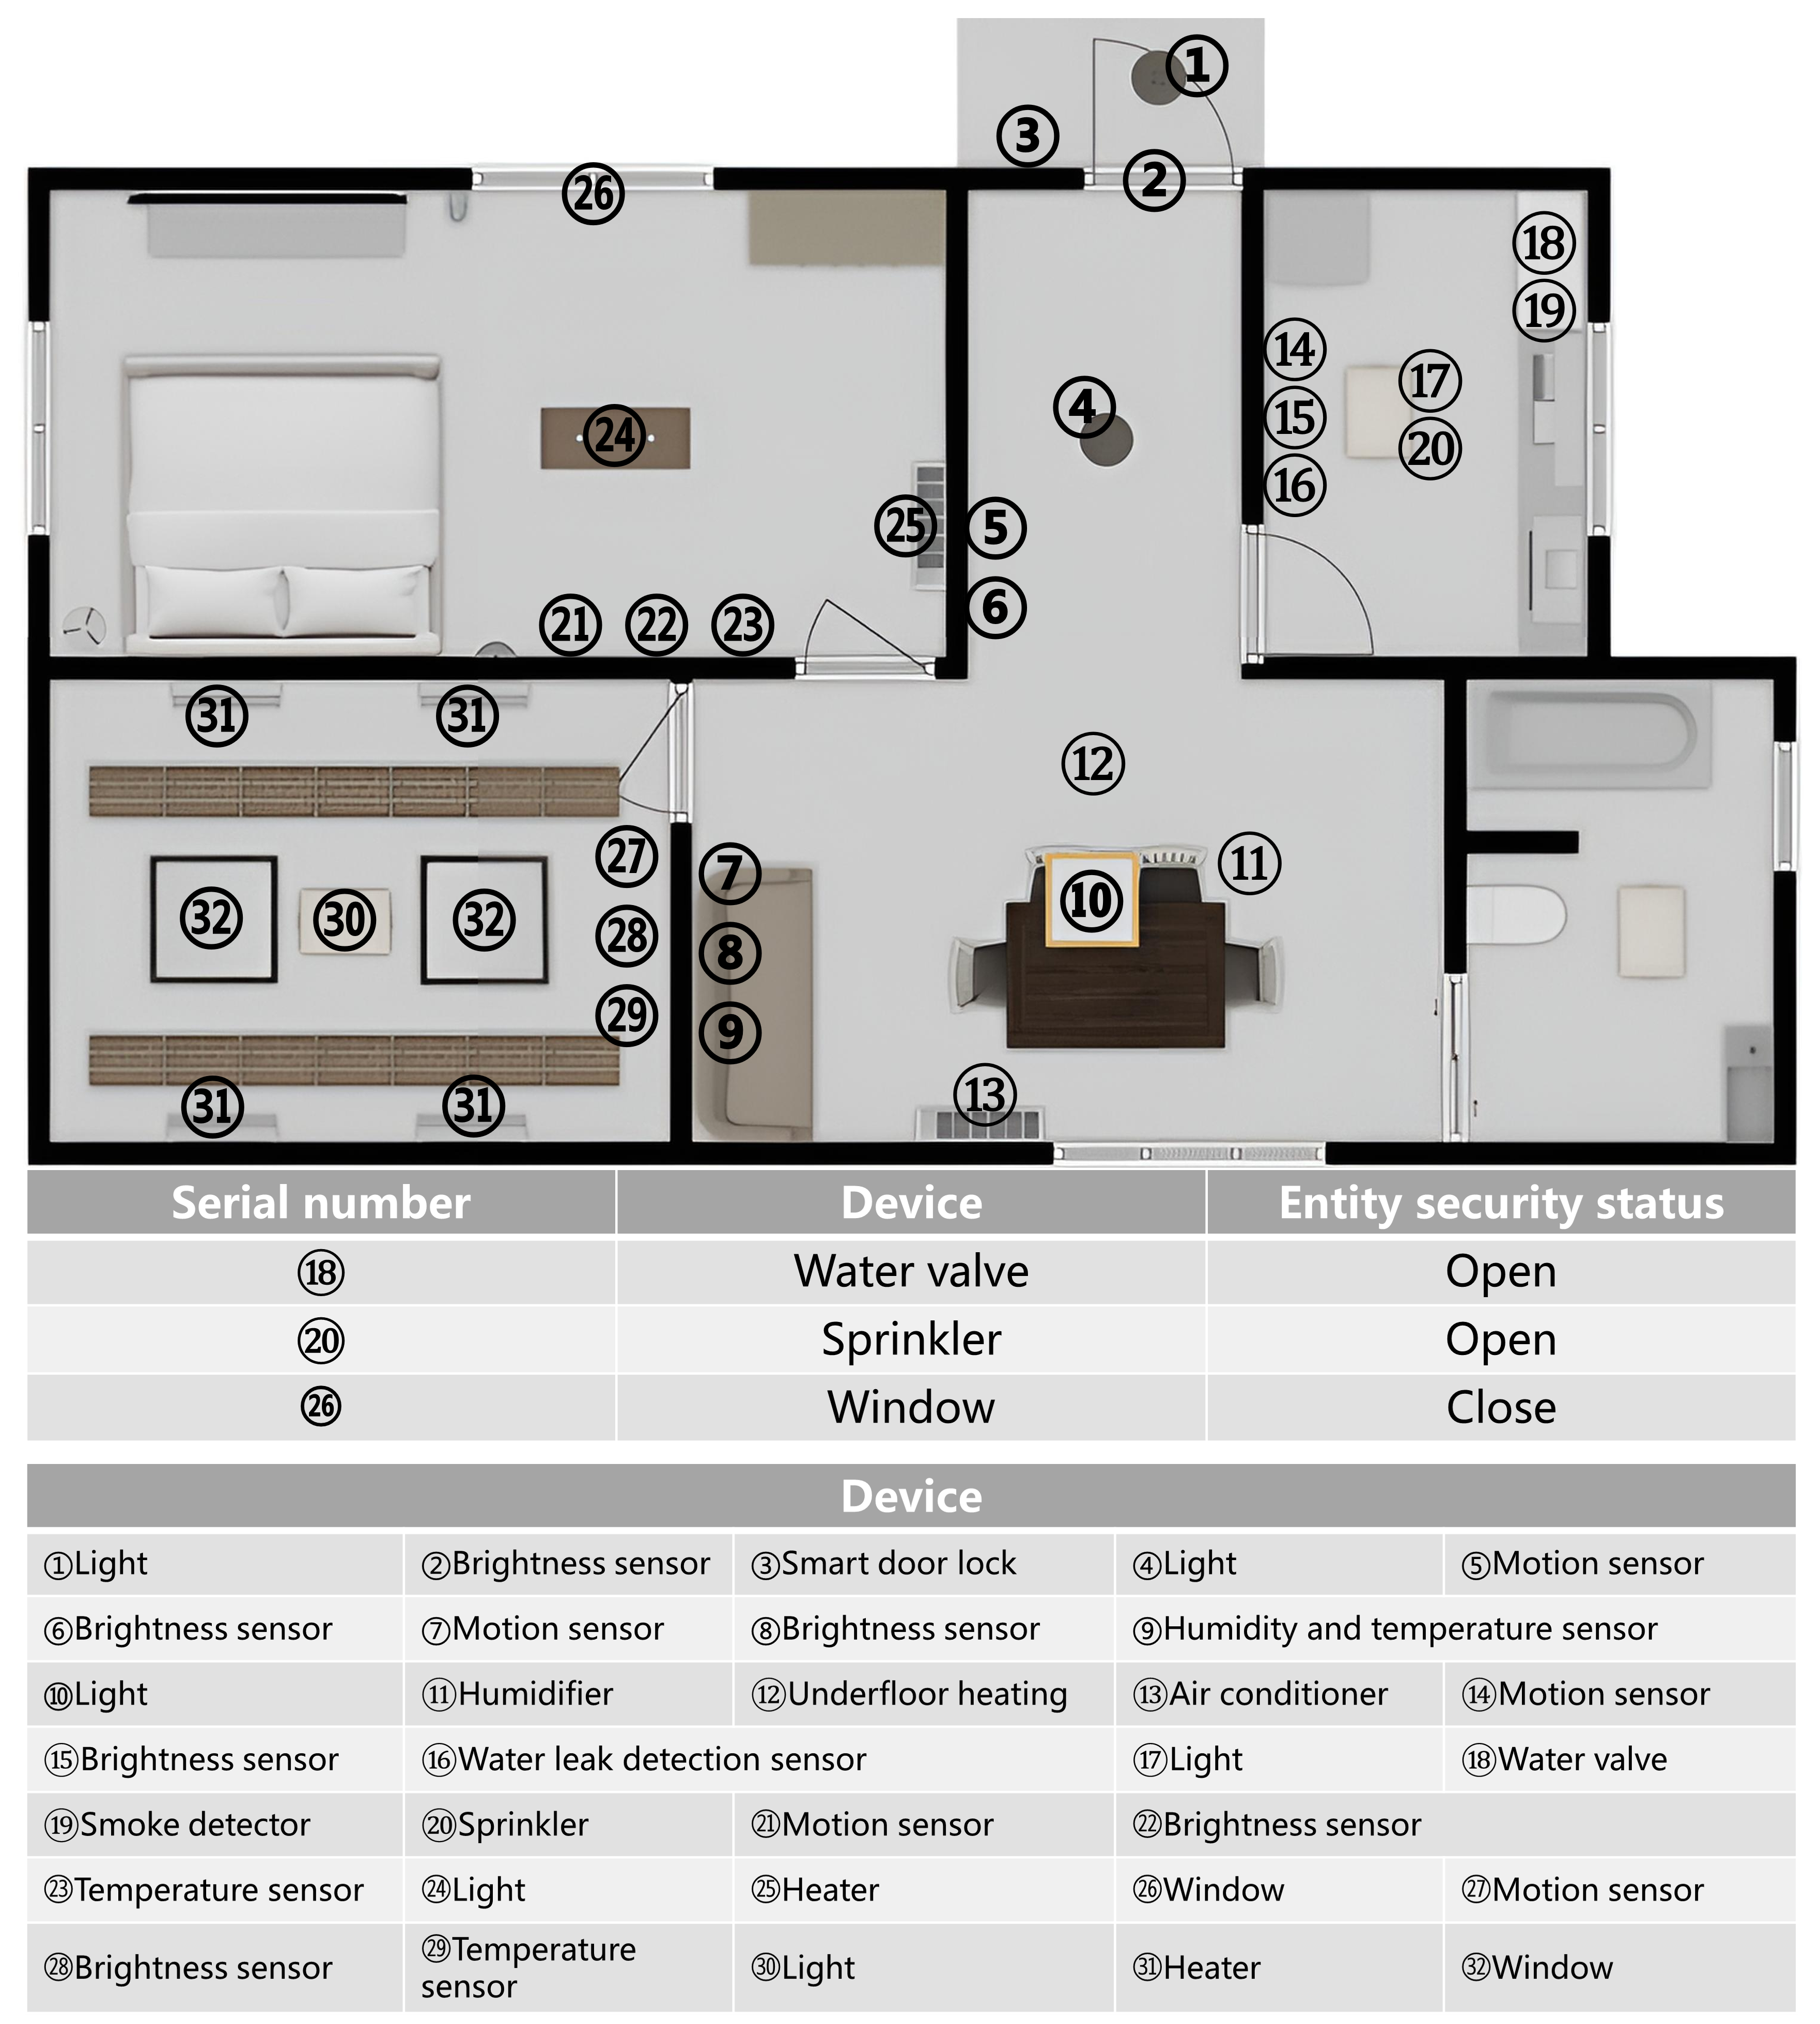
\includegraphics[width=0.5\textwidth]{figure/smarthome.png}
	\caption{Smart Home Floor Plan}
	\label{smarthome_floorplan}
\end{figure}

\subsection{Smart Home Testbeds}

%本文实现了一个完整的系统并进行了虚拟测试。对于虚拟测试,选择了基于 Python 的开源智能家居平台 Home Assistant。Home Assistant 支持来自各种制造商的设备,并提供虚拟设备以实现自动化功能。在此平台上,用户可以通过可视化 Web 界面或直接编辑配置文件来定义自定义自动化规则。Home Assistant 使用 YAML 配置文件来描述自动化规则,采用触发-条件-动作 (TCA) 模型。
This paper implements a complete system and conducts a virtual test. For the virtual test, Home Assistant, an open-source smart home platform based on Python, was selected.Home Assistant supports devices from various manufacturers and provides virtual devices to enable automation functionalities. On this platform, users can define custom automation rules either through a visual web interface or by directly editing configuration files. Home Assistant uses YAML configuration files to describe automation rules, employing a trigger-condition-action (TCA) model.

%虚拟测试使用图 \ref{smarthome_floorplan} 中所示的智能家居平面图。模拟的智能家居环境由七个不同的区域组成:室外、门廊、客厅、厨房、浴室、卧室和温室(花园)。根据观察,特定区域中的某些通道会相互影响。例如,门廊和客厅的亮度属性是相互依赖的,而客厅和卧室的亮度属性是独立的。
The virtual test uses the smart home floor plan illustrated in Figure \ref{smarthome_floorplan}. The simulated smart home environment consists of seven distinct zones: Outdoor, Porch, Living Room, Kitchen, Bathroom, Bedroom, and Greenhouse (Garden).  Based on observations, certain channels in specific zones can influence each other. For instance, the brightness attributes of the porch and living room are interdependent, while the brightness attributes of the living room and bedroom are independent.

%表 \ref{Testbeds} 列出了在这七个区域配置的 17 个自动化规则,以及相应的区域和设备。(附录 \ref{apdx:iot_devices} 显示了设备及其对应于区域的索引。)表 \ref{side_channel} 详细说明了智能家居系统中配置的侧通道,其中每个侧通道由一个区域、一个通道和一个趋势定义。最后,附录 \ref{apdx:iot_devices} 概述了智能家居系统中的实体安全配置,特别关注三个安全敏感设备的状态设置:水阀(开启)、喷水灭火器(开启)和卧室窗户(关闭)。
Table \ref{Testbeds} lists the 17 automation rules configured across these seven zones, along with the corresponding areas and devices. (Appendix \ref{apdx:iot_devices} shows the devices and their indices corresponding to the areas.) Table \ref{side_channel} details the side channels configured within the smart home system, where each side channel is defined by a zone, a channel, and a trend. Finally, Appendix \ref{apdx:iot_devices} outlines the entity security configurations in the smart home system, specifically focusing on the state settings for three security-sensitive devices: water valve (On), sprinkler (On), and bedroom window (Closed).

\begin{table}[htbp]
	\caption{Side Channel}
	\label{side_channel}
	\begin{tabular}[width=0.45\textwidth]{l|l|l}
		\hline
		\textbf{Area} & \textbf{Channel} & \textbf{Trend} \\
		\hline
		outdoor& brightness, & increase/decrease \\
		\hline
		porch& brightness, & increase/decrease \\
		\hline
		kitchen& brightness,temperature & increase/decrease \\
		\hline
		living room & brightness,humidity,temperature & increase/decrease \\
		\hline
		bedroom & brightness,temperature & increase/decrease \\
		\hline
		greenhouse & brightness,temperature & increase/decrease \\
		\hline
	\end{tabular}
\end{table}


\begin{table*}[htbp]
	\caption{Testbeds}
	\label{Testbeds}
	\centering
	\begin{adjustbox}{width=\textwidth}
	\begin{tabular}{c|l|c|l}
		\hline
		\textbf{Rule ID} & \textbf{Content} & \textbf{Area} & \textbf{Devices} \\
		\hline
		R1 & When the door lock is opened, if the brightness sensor is below 50lux, turn on the outdoor light and porch light. & Outdoor & \circled{1} \circled{2} \circled{3} \circled{4} \\
		\hline
		R2 & When the door lock is closed, turn off the porch light. & Outdoor & \circled{3} \circled{4} \\
		\hline
		R3 & When motion is detected in the porch, if the brightness sensor is below 50lux, turn on the porch light. & Porch & \circled{4} \circled{5} \circled{6} \\
		\hline
		R4 & When motion is detected in the living room, if the brightness sensor is below 50lux, turn on the living room light. & Living Room & \circled{7} \circled{8} \circled{10}\\
		\hline
		R5 & When the living room humidity is below 40\%, and the humidifier is off, turn on the living room humidifier. & Living Room & \circled{9} \circled{11} \\
		\hline
		R6 & When the living room humidity is above 60\%, turn off the living room humidifier. & Living Room & \circled{9} \circled{11} \\
		\hline
		R7 & When the living room temperature is below 24°C, turn off the living room floor heating and turn on the underfloor heating. & Living Room & \circled{9} \circled{12}\\
		\hline
		R8 & When the living room temperature is above 30°C, turn off the living room air conditioner and set it to 27°C. & Living Room & \circled{9} \circled{13} \\
		\hline
		R9 & When motion is detected in the kitchen, if the brightness sensor is below 50lux, turn on the kitchen light. & Kitchen & \circled{14} \circled{15} \circled{17} \\
		\hline
		R10 & When a water leak is detected, close the main water valve. & Kitchen & \circled{16} \circled{18} \\
		\hline
		R11 & When the smoke detector is triggered, turn on the sprinkler. & Kitchen & \circled{19} \circled{20} \\
		\hline
		R12 & When motion is detected in the bedroom, if the brightness sensor is below 50lux, turn on the bedroom light. & Bedroom & \circled{21} \circled{22} \circled{24} \\
		\hline
		R13 & At 7 PM, turn on the bedroom heating. & Bedroom & \circled{25} \\
		\hline
		R14 & When the bedroom temperature reaches 30°C, open the window and close the heating. & Bedroom & \circled{23} \circled{25} \circled{26} \\
		\hline
		R15 & When motion is detected in the green house, if the brightness sensor is below 50lux, turn on the green house light. & Green house & \circled{27} \circled{28} \circled{30}\\
		\hline
		R16 & At 7 PM, turn on the green house heating. & Green house & \circled{31} \\
		\hline
		R17 & When the green house temperature reaches 32°C, open the window and close the heating. & Green house & \circled{29} \circled{31} \circled{32} \\
		\hline
	\end{tabular}
	\end{adjustbox}
\end{table*}

\subsection{Effectiveness of Conflict Detection}
%为了评估规则冲突的检测有效性,采用手动触发的方式测试所有可能的规则交互,并手动检测出其中存在的四条规则冲突,每条规则冲突可能对应多种规则冲突类型,然后使用本论文实现的系统进行静态检测与动态检测(同样采用手动触发的方式),同时对比了IoTMEDIATOR的检测结果。
In order to evaluate the effectiveness of rule conflict detection, all possible rule interactions were tested using manual triggering, and four rule conflicts were identified(Each rule conflict can correspond to multiple rule conflict types). Subsequently, the system implemented in this paper was used for both static and dynamic detection (also through manual triggering), while also comparing the detection results with those of IoTMEDIATOR.

%所有七个区域的17条规则的冲突测试结果如Table.\ref{conflict_detection_result}所示,其中R10-R11存在规则冲突:R10会控制水阀关闭,导致在R11被触发时,R11无法正常执行。R11-R10存在规则冲突:R11执行时,会触发R10的执行,且R11的执行动作与R10的执行动作互斥。R13-R14存在规则冲突:R13的执行会触发R14的执行,且两条规则的执行动作互斥。R14-R13存在规则冲突:R14的执行结果与R13的执行结果互斥。
The conflict results of 17 rules in all seven regions are shown in Table.\ref{conflict_detection_result}. Among them, there is a conflict between R10 and R11: R10 controls the water valve to close, causing R11 to fail execution when triggered. There is also a conflict between R11 and R10: when R11 is executed, it triggers the execution of R10, and the execution actions of R11 and R10 are mutually exclusive. Additionally, there is a conflict between R13 and R14: the execution of R13 triggers the execution of R14, and the execution actions of both rules are mutually exclusive. There is also a conflict between R14 and R13: the execution result of R14 is mutually exclusive with that of R13.

%测试结果表示IoTMEDIATOR能够检测到其中的R11-R10、R13与R14与R14-R13的规则冲突,而无法检测到R10与R11通过humidity的side channel互相影响导致的规则冲突,即智能家居系统检测到漏水后关闭水阀,此后如果用户没有及时处理,如果引发火灾,水阀仍旧没有开启,R11无法正常执行。同时IoTMEDIATOR坚持到了许多其他的规则交互,但是他们是否属于规则冲突需要用户进行根据主观偏好进行选择。例如:规则 R5 控制客厅加湿器以增加湿度,而规则 R6 控制加湿器以关闭以防止湿度过高。这两条规则之间的交互能够便捷地维持客厅湿度,不应被视为规则冲突。(IoTMEDIATOR对于Race Condition、 Potential Race Condition和Condition Bypass时对称的,即两条规则对应两次规则冲突,在表格中可能只展示一次,后续需要修改——zyd)
The test results indicate that IoTMEDIATOR is able to detect the rule conflicts of R11-R10, R13 with R14, and R14-R13, but it fails to detect the rule conflict caused by the mutual influence through humidity between R10 and R11. Specifically, after the smart home system shuts off the water valve upon detecting a water leak, if the user does not respond in time and a fire is triggered, the water valve will not open, resulting in R11 not executing normally. Meanwhile, IoTMEDIATOR persists with many other rule interactions; however, whether they constitute rule conflicts is subject to the user's subjective preference. For example, R5 controls the living room humidifier to increase humidity, while R6 controls the humidifier to shut off in order to prevent excessive humidity. The interaction between these two rules conveniently maintains the living room’s humidity and should not be regarded as a conflict.

%所有规则交互都能被我们的系统精确捕捉,同时能够自动将任何威胁性规则交互是为规则冲突,从而检测到所有的四条规则冲突,并检测出六种可能的冲突发生方式。除此之外,我们的系统能够有效避免规则冲突的误报,极大程度上避免了将正常的规则交互错误分类到规则冲突的可能性,与此同时用户可以将其他规则交互根据个人偏好选择是否列入规则冲突列表中。
All rule interactions can be precisely captured by our system, and it is capable of automatically converting any threatening rule interactions into rule conflicts, thereby detecting all four types of rule conflicts and identifying six possible ways in which conflicts might occur. In addition, our system effectively avoids false positives in identifying rule conflicts, greatly minimizing the chance that normal rule interactions are mistakenly classified as conflicts, while also allowing users to optionally include other rule interactions in the rule conflict list according to their personal preference.

\begin{table*}[htbp]
	\centering
	\caption{Result of Rule Conflict Detection}
	\label{conflict_detection_result}
	\begin{adjustbox}{width=\textwidth}
	\begin{tabular}{|c|l|c|c|c|c|c|c|c|c|c|c|c|c|c|c|c|c|c|c|c|c|c|}
		\hline
		& \textbf{Classification} & \textbf{R1-R2} & \textbf{R1-R3} & \textbf{R1-R4} & \textbf{R1-R9} & \textbf{R2-R3} & \textbf{R2-R4} & \textbf{R2-R12} & \textbf{R3-R4} & \textbf{R3-R9} & \textbf{R4-R3} & \textbf{R5-R6} & \textbf{R6-R5} & \textbf{R7-R8} & \textbf{R8-R7} & \textbf{R9-R3} & \textbf{R10-R11} & \textbf{R11-R10} & \textbf{R13-R14} & \textbf{R14-R13} & \textbf{R15-R12} & \textbf{R16-R17} \\ \hline
		\multirow{6}{*}{\rotatebox{90}{Ours}} & Trigger Conflict &  &  &  &  &  &  &  &  &  &  &  &  &  &  &  &  &  &  &  &  &  \\ 
		\cline{2-23}
		& Condition Conflict &  &  &  &  &  &  &  &  &  &  &  &  &  &  &  &  &  &  &  &  &  \\ 
		\cline{2-23}
		& Action Conflict &  &  &  &  &  &  &  &  &  &  &  &  &  &  &  &  &  & \checkmark & \checkmark &  &  \\ 
		\cline{2-23}
		& Indirect Trigger Conflict &  &  &  &  &  &  &  &  &  &  &  &  &  &  &  &  & \checkmark & \checkmark &  &  &  \\ 
		\cline{2-23}
		& Indirect Condition Conflict &  &  &  &  &  &  &  &  &  &  &  &  &  &  &  &  &  &  &  &  &  \\ 
		\cline{2-23}
		& Indirect Action Conflict &  &  &  &  &  &  &  &  &  &  &  &  &  &  &  & \checkmark & \checkmark &  &  &  &  \\
		 \cline{2-23}
		\hline
		\multirow{7}{*}{\rotatebox{90}{IoTMediator}} 
		& Condition Enabling/Disabling &  & \checkmark & \checkmark & \checkmark & \checkmark & \checkmark & \checkmark & \checkmark & \checkmark & \checkmark & \checkmark & \checkmark &  &  & \checkmark &  &  &  &  & \checkmark &  \\ 
		\cline{2-23}
		& Race Condition &  &  &  &  &  &  &  &  &  &  &  &  &  &  &  &  &  &  &  &  &  \\ 
		\cline{2-23}
		& Potential Race Condition & \checkmark &  &  &  & \checkmark &  &  &  &  &  & \checkmark &  &  &  &  &  &  &  &  &  & \checkmark \\
		\cline{2-23}
		& Chained Execution &  &  &  &  &  &  &  &  &  &  & \checkmark & \checkmark & \checkmark & \checkmark &  &  & \checkmark & \checkmark &  &  & \checkmark \\ 
		\cline{2-23}
		& Action Revert &  &  &  &  &  &  &  &  &  &  & \checkmark & \checkmark &  &  &  &  &  & \checkmark &  &  & \checkmark \\ 
		\cline{2-23}
		& Infinite Loop &  &  &  &  &  &  &  &  &  &  & \checkmark & \checkmark & \checkmark & \checkmark &  &  &  &  &  &  &  \\ 
		\cline{2-23}
		& Condition Bypass &  &  &  &  &  &  &  &  &  &  &  &  &  &  &  &  &  &  &  &  &  \\ \hline
	\end{tabular}
	\end{adjustbox}
\end{table*}

\subsection{Availability of Automated Rule Conflict Resolution}

\begin{figure}[htbp]
	\centering
	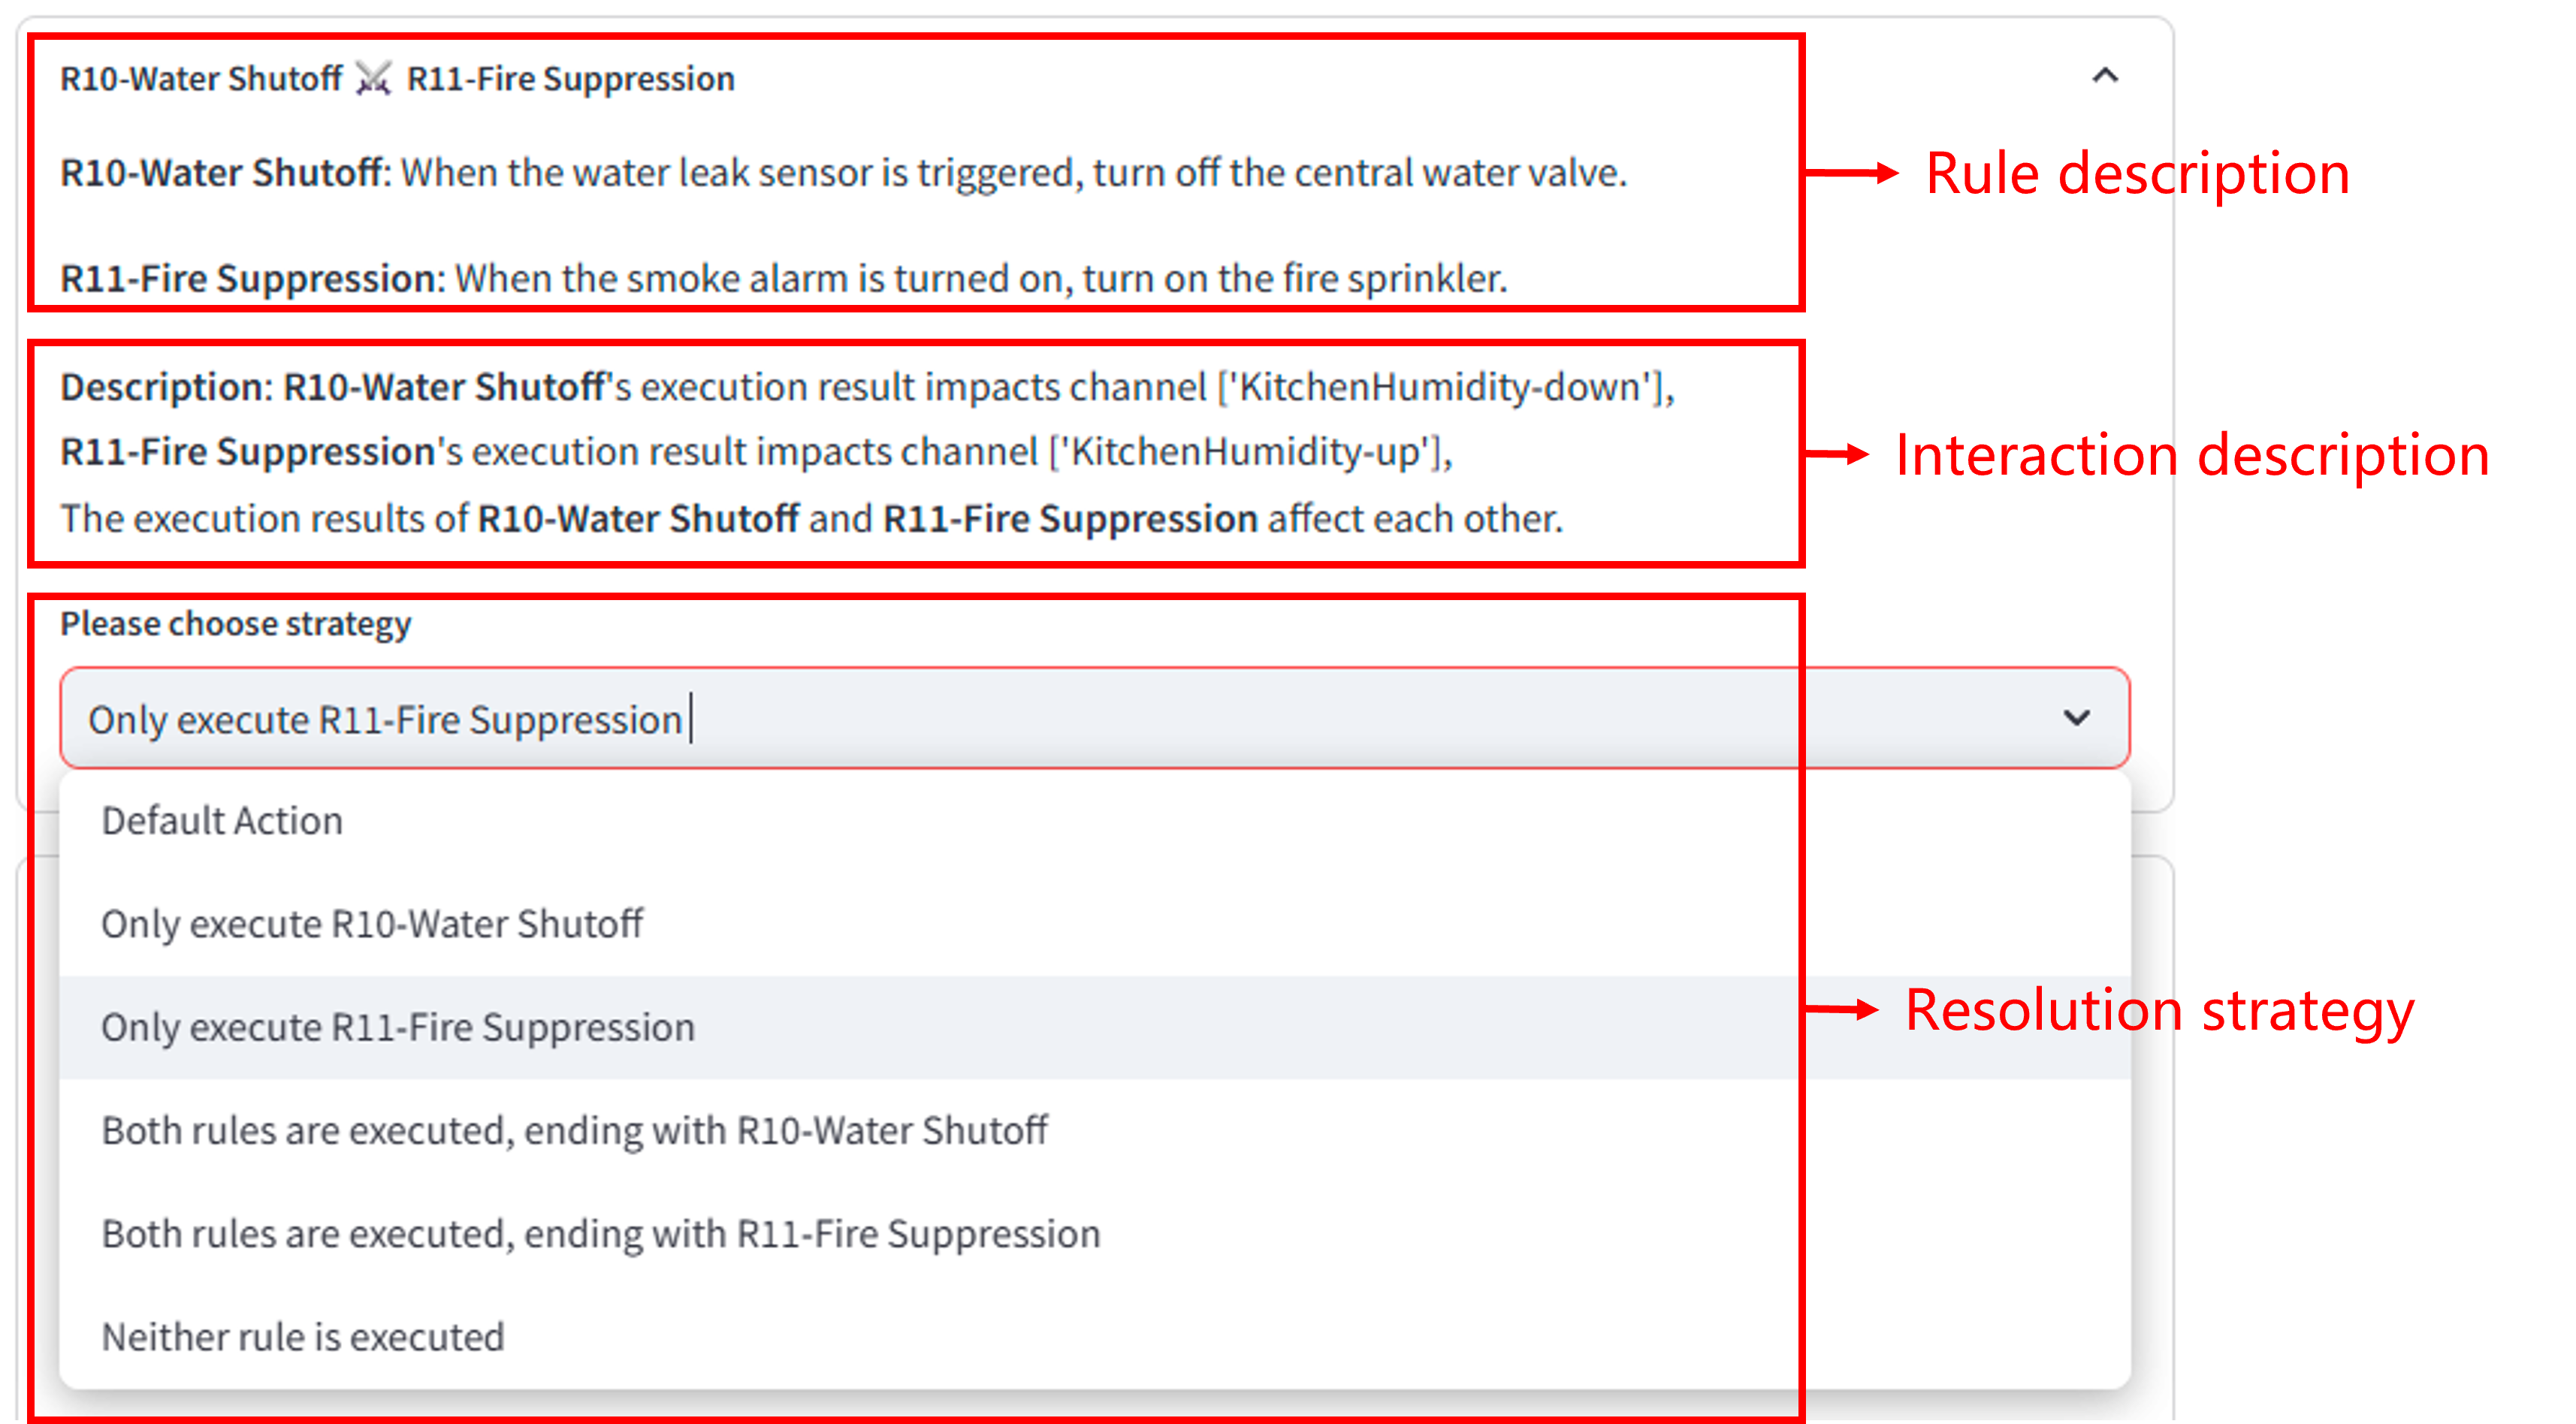
\includegraphics[width=0.45\textwidth]{figure/resolution_example.png}
	\caption{Example of Automated Rule Conflict Resolution}
	\label{example_resolution}
\end{figure}

%为了评估自动化的规则冲突处理的可用性,本章节将结合具体的示例展示对于一个具体的规则冲突,系统如何进行自动化处理,以及AI对于系统提供的规则冲突信息的推测处理方式。
In order to assess the applicability of automated rule conflict resolution, this chapter will use specific examples to demonstrate how the system automatically processes a particular rule conflict and how AI speculatively handles the rule conflict information provided by the system.

%Fig.\ref{example_resolution}展示了规则R10与规则R11对应的Indirect Action Conflict。图片中展示了规则的描述(自动化规则配置文件中提取得到),规则冲突描述(Rule Conflict Detection Module中根据上下文信息生成)为:R10-Water Shutoff's execution result impacts channel ['KitchenHumidity-down'],R11-Fire Suppression's execution result impacts channel ['KitchenHumidity-up'],The execution results of R10-Water Shutoff and R11-Fire Suppression affect each other.最下面是处理策略,包含一个默认执行动作和五个规则冲突缓解动作。
Fig.\ref{example_resolution} displays the Indirect Action Conflict corresponding to rules R10 and R. The image shows the description of the rules (extracted from the automated rule configuration file) and the rule conflict description (generated by the Rule Conflict Detection Module based on contextual information) as: R10-Water Shutoff's execution result impacts channel ['KitchenHumidity-down'], R11-Fire Suppression's execution result impacts channel ['KitchenHumidity-up'], and the execution results of R10-Water Shutoff and R11-Fire Suppression affect each other. At the bottom is the resolution strategy, which consists of a default execution action and five rule conflict mitigation actions.

%根据实体安全配置,规则R10的执行动作将水阀关闭,使用线性函数进行评估,其对应的安全值参数$sf_{R10}=-1$,而R11的执行动作将开启消防喷淋头,其对应的安全值参数$sf_{R11}=1$,因此Generation of Resolution Strategy Module将会自动化推荐“Only excute R11”策略用于预防规则冲突的真实发生。除此之外页面的对处理策略提供选项,用户可以对规则冲突处理策略进行选择,以选择更符合偏好的处理方案。
According to the entity security configuration, the execution action of rule R10 will close the water valve, and its evaluation is conducted using a linear function with the corresponding safety parameter $sf_{R10}=-1$, while the execution action of rule R11 will activate the fire sprinkler head, with its corresponding safety parameter $sf_{R11}=1$. Therefore, the Generation of Resolution Strategy Module will automatically recommend the "Only execute R11" strategy to prevent real conflicts between rules. In addition, the page provides options for resolution strategies, allowing users to choose a rule conflict resolution strategy that better fits their preferences.

%为了测试Rule Conflict Detection Module根据规则模型生成的规则冲突描述对用户的友好性,本论文使用AI测试其对规则冲突的处理策略选择。仍旧以Fig.\ref{example_resolution}为例,使用的模型为gpt-4o-2024-11-20,调用方式为OPENAI API,其它参数默认不做修改,系统提示词将会展示在 Appendix.\ref{apdx:system_prompt}。对于上述示例我们得到的回复如下:\texttt{\{
%		"policy": "2", // Only execute R11
%		"reason": "In this case of Indirect Rule Action Conflict, the sprinkler system activated by R11 is crucial for safety during a fire, and its priority should supersede the water cutoff triggered by R10 to ensure effective fire suppression. Therefore, only R11 should execute."
%	\}}
To test the user-friendliness of the rule conflict description generated according to the rule model by the Rule Conflict Detection Module, this paper uses AI to test its strategy selection for conflict resolution. Still taking Fig.\ref{example_resolution} as an example, the model used is \texttt{gpt-4o-2024-11-20}, called via the OPENAI API, with other parameters remaining unchanged by default, and the system prompt will be shown in Appendix.\ref{apdx:system_prompt}. For the above example, we obtained the following response: 
\texttt{\{\\
	"policy": "2", // Only execute R11 \\
	"reason": "In this case of Indirect Rule Action Conflict, the sprinkler system activated by R11 is crucial for safety during a fire, and its priority should supersede the water cutoff triggered by R10 to ensure effective fire suppression. Therefore, only R11 should execute."\\
	\}}\\

%通过AI对规则冲突描述的理解对规则冲突处理策略的推荐结果与预期相契合,一定程度上标明当前的提取的规则冲突信息能够很好地被用户理解,并作出正确有效的选择,也为用户提供了使用智能工具进行规则冲突处理策略推荐的选择。
Through AI's understanding of rule conflict descriptions, the recommended results for rule conflict resolution strategies align with expectations, which to some extent indicates that the currently extracted rule conflict information can be well understood by users, enabling them to make correct and effective choices, and providing them with the option to use intelligent tools for recommending rule conflict resolution strategies.

\subsection{Performance} 
%为了测试系统性能,本论文根据系统架构将测试分为静态分析的性能评估与动态检测与冲突处理的性能评估。
In order to test the system performance, this paper divides the testing into performance evaluation of static analysis and performance evaluation of dynamic detection and conflict based on the system architecture.

%其中静态检测的性能评估中,静态检测会遍历所有的自动化规则(包含Formal Analysis Module和Rule Conflict Detection Module),并对每两种规则进行比较,还将进行自比较,因此对于n条规则来说,静态检测的时间复杂度为$O\left(n^2\right)$。对于测试使用Testbeds规则集(17条),AI生成的100条规则集(100条)与1000条规则集(1000条)作为输入评估多次检测耗时,单位为秒,为便于展示选择其中三次检测结果并记录平均值,Table.\ref{performance_static_detection}展示了测试的结果。可以观察到Testbeds中的17条规则,静态检测耗时仅需要$3.5ms$,即使存在1000条规则,静态检测也只需要约$12s$,不同数据量的静态检测耗时符合预期的复杂度。
In the performance evaluation of static analysis(Contains Formal Analysis Module and Rule Conflict Detection Module), the static analysis traverses all the automation rules and compares each pair of rules, including self-comparison. Therefore, for n rules, the time complexity of static detection is $O\left(n^2\right)$. For testing, the Testbeds rule set (17 rules), an AI-generated 100-rule set (100 rules), and a 1000-rule set (1000 rules) were used as inputs to evaluate the detection time multiple times, in seconds. To facilitate the display, three analysis results were selected and the average value was recorded. Figure.\ref{performance_static_analysis} shows the test results. It can be observed that the static detection of the 17 rules in Testbeds only takes $3.5ms$. Even with 1000 rules, static analysis only takes about $12s$, and the static analysis time of different data volumes meets the expected complexity.

%\begin{table}[htbp]
%	\caption{Performance of Static Detection}
%	\label{performance_static_detection}
%	\centering
%	\begin{tabular}[width=1\textwidth]{|c|c|c|c|c|}
%		\hline
%		Number of Rules & 1st  & 2nd & 3rd  & Average Time \\
%		\hline
%		10 & $ 1.509 \times 10^{-3}$ & $0.997 \times 10^{-3}$ & $1.505 \times 10^{-3}$ & $1.337 \times 10^{-3}$ \\
%		\hline
%		17 & $4.002 \times 10^{-3}$ & $2.998 \times 10^{-3}$ & $3.508 \times 10^{-3}$ & $3.503 \times 10^{-3}$ \\
%		\hline
%		50 & $2.817 \times 10^{-2}$ & $2.952 \times 10^{-2}$ & $2.952 \times 10^{-2}$ & $2.907 \times 10^{-2}$ \\
%		\hline
%		100 & $1.193 \times 10^{-1}$ & $1.162 \times 10^{-1}$ & $1.188 \times 10^{-1}$ & $1.181 \times 10^{-1}$ \\
%		\hline
%		500 & $3.003 $ & $2.997$ & $2.974$ & $2.991$ \\
%		\hline
%		1000 & $1.190 \times 10^{1}$ & $1.191 \times 10^{1}$ & $1.205 \times 10^{1}$ & $1.195 \times 10^{1}$ \\
%		\hline
%	\end{tabular}
%	
%\end{table}

\begin{figure}[htbp]
	\caption{Performance of Static Analysis}
	\label{performance_static_analysis}
	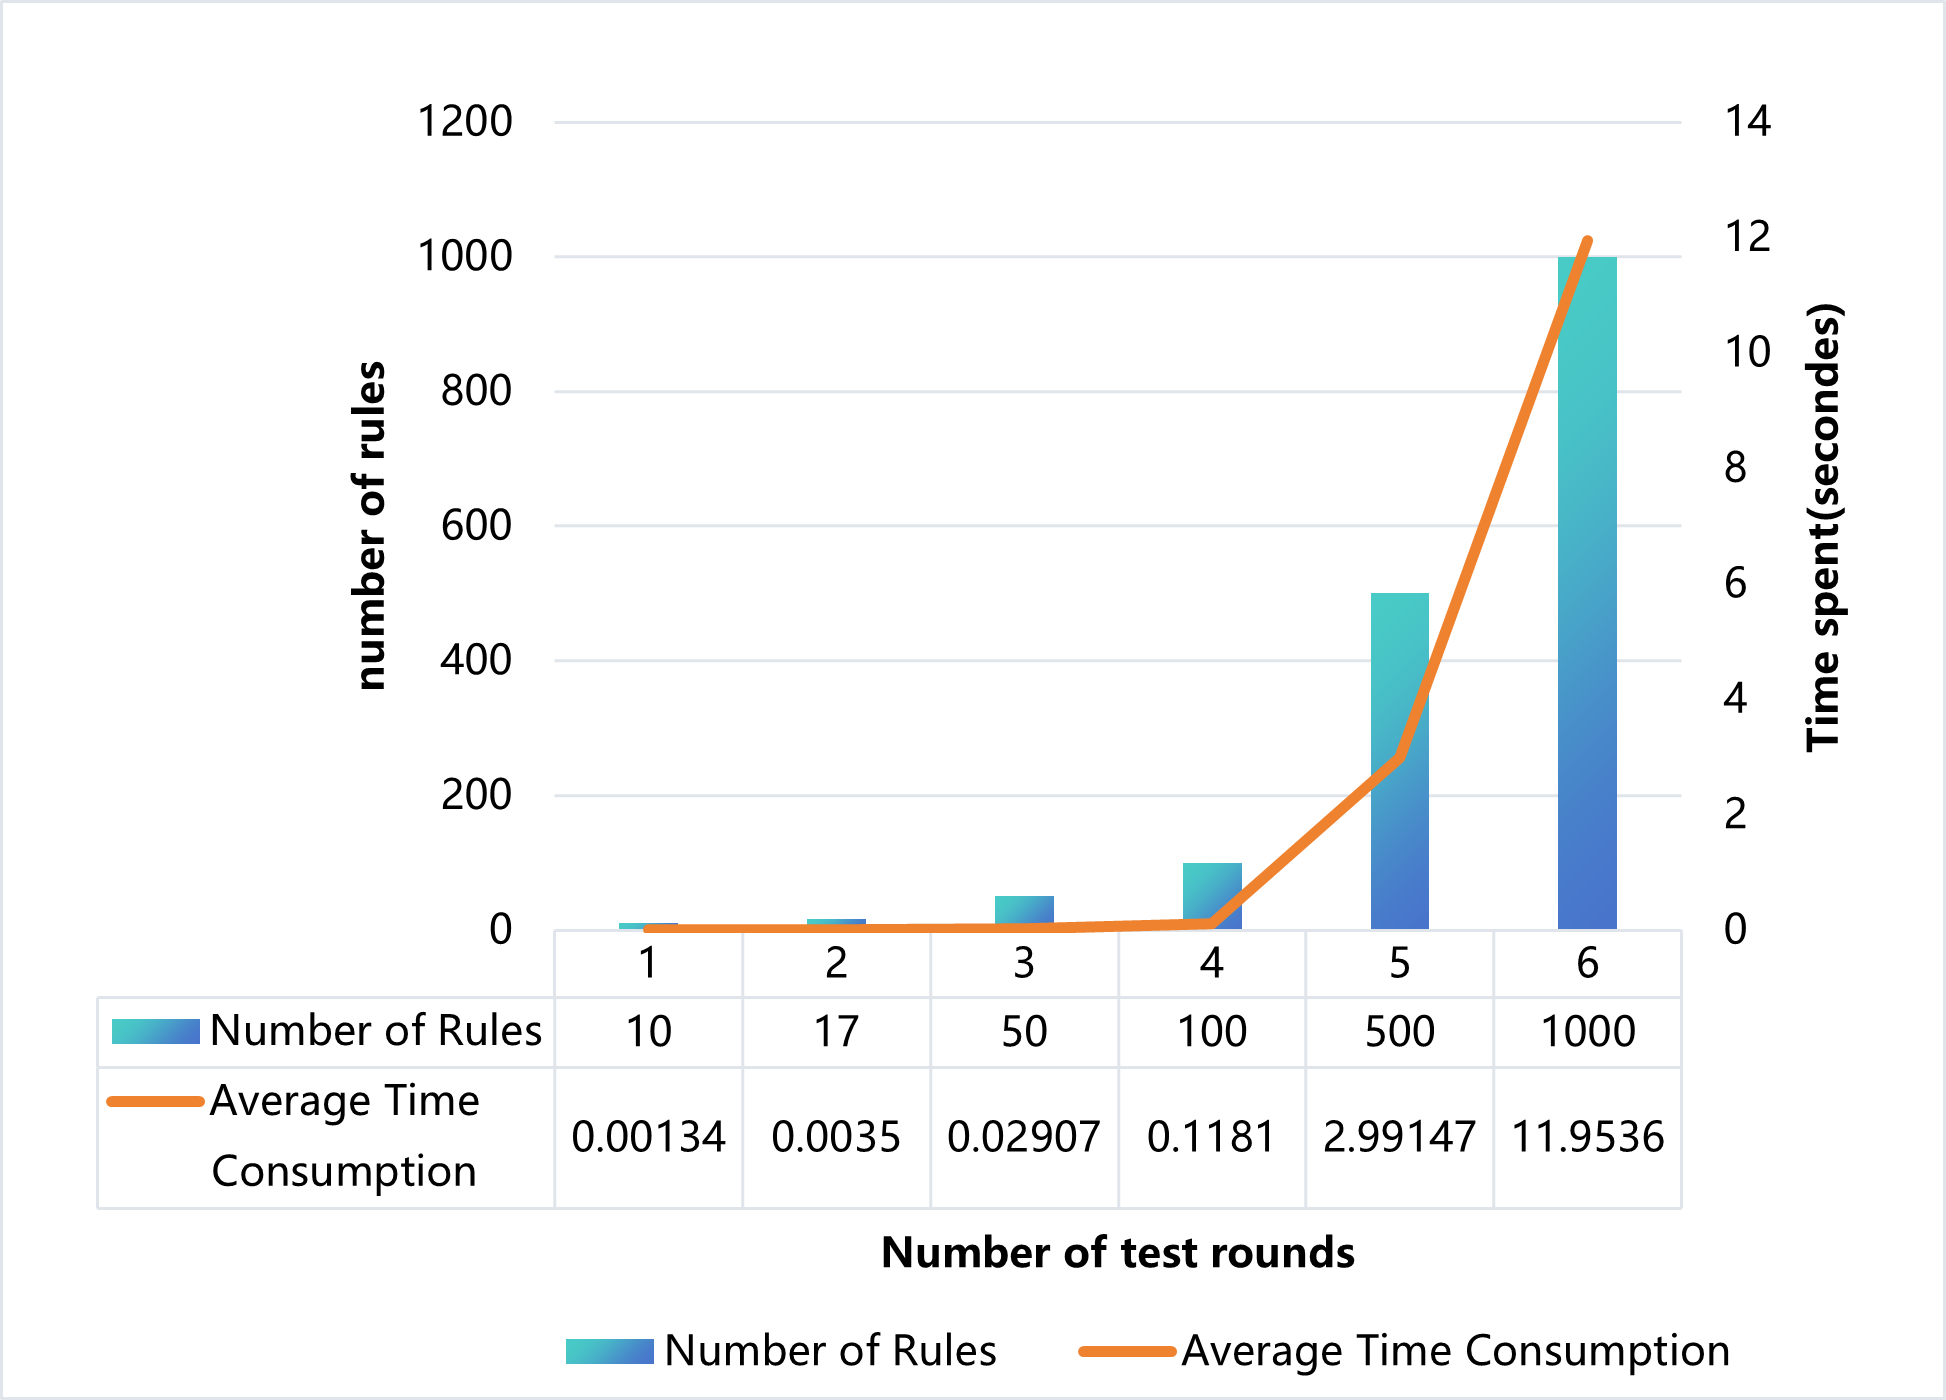
\includegraphics[width=0.5\textwidth]{figure/performance.png}
	
\end{figure}

%在规则冲突动态检测(Assertion Verification Module)与规则冲突处理指令生成(Command Generation Module)两个模块中,其本身计算量不高,时间消耗主要体现在通信过程,因此接下来着重进行代码插桩装通信性能评估,测试包括随机触发规则冲突,对所有通信函数(包括系统发送消息,Home Assistant平台处理完毕返回消息,系统接收到消息三个阶段)的性能测评,通信函数的介绍与性能测评结果如Table.\ref{performance_communication_function}所示。
In the two modules—the Assertion Detection Module for detecting rule conflicts dynamically and the Command Generation Module for handling rule conflict processing—the computational load is not high, and the time consumption mainly lies in the communication process. Therefore, the focus will next be on code instrumentation for communication performance evaluation, testing which includes randomly triggering rule conflicts and assessing the performance of all communication functions (covering the three stages of system sending messages, Home Assistant platform processing and returning messages, and system receiving messages). The introduction and performance evaluation results of the communication functions are shown in Table.\ref{performance_communication_function}.

%可以观察到在实验环境中的通信函数平均与最长耗时仅有毫秒级别,且在断言验证与规则冲突处理方案指令生成两个步骤中只会调用有限次数的通信函数,且耗时均也只有毫秒级别。
It can be observed that the average and maximum time consumption of the communication functions in the experimental environment are only at the millisecond level, and that only a limited number of calls are made to the communication functions during the two steps of assertion verification and rule conflict handling directive generation, with each call also taking only a few milliseconds.

\begin{table*}[htpb]
	\caption{Performance of Communication Functions}
	\label{performance_communication_function}
	\centering
	\begin{tabular}{c|c|c|c}
		\hline
		\textbf{Function Name} & \textbf{Description} & \textbf{Average Time Consumption} & \textbf{Maximum Time Consumption}\\
		\hline
		get\_entity\_state & Get entity state & $1.193 \times 10^{-3}$s & $1.953 \times 10^{-3}$s \\
		\hline
		time\_now & Get HomeAssistant system time & $9.765 \times 10^{-4}$s & $9.825 \times 10^{-4}$s \\
		\hline
		command\_send & Send conflict handling command & $9.643 \times 10^{-4}$s & $9.787 \times 10^{-4}$s \\
		\hline
		communicate\_finish & End communication phase & $9.778 \times 10^{-4}$s & $9.832 \times 10^{-4}$s \\
		\hline
		\multicolumn{4}{l}{Note: Each function is tested 10 times.} \\
	\end{tabular}
\end{table*}
\section{Limitations and Discussion}
\section{Related Work}
\section{Conclusion}

\bibliographystyle{ieeetr}
\bibliography{paper}
\appendices
\section{System Prompt}
\label{apdx:system_prompt}
\texttt{
	You are a smart home expert who can handle conflicts in automation rules in smart home life.
	Rule conflicts are divided into the following types: ['Rule Action Conflict', 'Rule Trigger Conflict', 'Rule Condition Conflict', 'Indirect Rule Trigger Conflict', 'Indirect Rule Condition Conflict', 'Indirect Rule Action Conflict'];\\
	There are several types of rule conflicts:{'Rule Action Conflict': 'The execution actions of two rules conflict', 'Rule Trigger Conflict': 'The execution of rule i causes the rule to be triggered', 'Rule Condition Conflict': 'The execution of rule i prohibits or allows the conditions of rule j', 'Indirect Rule Trigger Conflict': 'The impact of rule i on the other channel unexpectedly causes rule j to be triggered', 'Indirect Rule Condition Conflict': 'The impact of the execution of rule i on the other channel causes the conditions of rule j to be allowed or disabled', 'Indirect Rule Action Conflict': 'Two rules interact with two different devices that affect the same channel property'};\\
	For Rule Action Conflict, when multiple rules set different values for the same device at the same time, the device status will be updated according to the order in which the rules are executed.
	Pay attention to the index order starting from 0, `R1` represents the first rule in the rule pair, often indicating the rule that is executed first in the rule pair. `R2` represents the second rule in the rule pair, often indicating the rule that is executed later in the rule pair. `R1` and `R2` respectively refer to the chat rules given by the user in sequence.\\
	For conflicts of type Rule Action Conflict and Indirect Rule Action Conflict, the conflict resolution strategies and their indexes are as follows: {'Default Action': 0, 'Only execute {R1}': 1, 'Only execute {R2}': 2, 'Both rules are executed, ending with {R1}': 3, 'Both rules are executed, ending with {R2}': 4, 'Neither rule is executed': 5};\\
	For conflicts of type Rule Trigger Conflict and Indirect Rule Trigger Conflict, the conflict resolution strategies and their indexes are as follows: {'Default Action': 0, 'Only execute {R2}': 1, 'Default execution {R2}': 2, 'Cancel execution of {R2}': 3};\\
	For conflicts of type Rule Condition Conflict and Indirect Rule Condition Conflict, the conflict resolution strategies and their indexes are as folloThe format of the data provided by the user is as follows:\\
	```
	Information about the first rule, including the rule name and id, rule content <trigger | condition | action>, and rule description\\
	Information about the second rule, including the rule name and id, rule content <trigger | condition | action>, and rule description\\
	Description of rule violation\\
	```
	The rules are given in the order of triggering execution, that is, the rules given first are executed first. The time interval between the execution of two rules may be very short, triggered almost at the same time, or it may be a long time, please consider the reasons for rule conflict and select an appropriate conflict resolution strategy based on the type of rule conflict and actual situation, thinking from the user's perspective while addressing resources and protecting the safety of the family, and give indicators and rationale for the appropriate resolution strategy.
	For example, to prevent unintended opening of doors and windows due to rule conflicts/rule interactions, and to water valves from being shut off during a fire.\\
	Your response should be directly in the following JSON structure, not in markdown format, without any extra explanation and code block:\\
	\{\\
	'policy': "index of policy",\\
	'reason': "reason why you choose this policy"\\
	\}
}

\section{IoT Devices}
\label{apdx:iot_devices}
\begin{table}[htbp]
	\caption{IoT Devices}
	\begin{adjustbox}{width=0.5\textwidth}
	\begin{tabular}[width=0.5\textwidth]{c|c|c|c}
		\hline
		\textbf{Area} & \makecell{\textbf{Serial} \\ \textbf{number}} & \textbf{Devices} & \makecell{\textbf{Entity security} \\ \textbf{status}} \\
		\hline
		\multirow{3}{*}{Outdoor}& \circled{1} & Light &\diagbox{}{}  \\
		\cline{2-4}
		& \circled{2} & Brightness sensor &\diagbox{}{} \\
		\cline{2-4}
		& \circled{3} & Smart door lock &\diagbox{}{} \\
		\hline
		
		\multirow{3}{*}{Porch}& \circled{4} & Light &\diagbox{}{} \\
		\cline{2-4}
		& \circled{5} & Motion sensor &\diagbox{}{} \\
		\cline{2-4}
		& \circled{6} & Brightness sensor &\diagbox{}{} \\
		\hline
		
		\multirow{7}{*}{Living room}& \circled{7} & Motion sensor &\diagbox{}{} \\
		\cline{2-4}
		& \circled{8} & Brightness sensor &\diagbox{}{} \\
		\cline{2-4}
		& \circled{9} & Humidity and temperature sensor &\diagbox{}{} \\
		\cline{2-4}
		& \circled{10} & Light &\diagbox{}{} \\
		\cline{2-4}
		& \circled{11} & Humidifier &\diagbox{}{} \\
		\cline{2-4}
		& \circled{12} & Underfloor heating &\diagbox{}{} \\
		\cline{2-4}
		& \circled{13} & Air conditioner &\diagbox{}{} \\
		\hline
		
		\multirow{7}{*}{Kitchen}& \circled{14} & Motion sensor &\diagbox{}{} \\
		\cline{2-4}
		& \circled{15} & Brightness sensor &\diagbox{}{} \\
		\cline{2-4}
		& \circled{16} & Water leak detection sensor &\diagbox{}{} \\
		\cline{2-4}
		& \circled{17} & Light &\diagbox{}{} \\
		\cline{2-4}
		& \circled{18} & Water valve & Open \\
		\cline{2-4}
		& \circled{19} & Smoke detector &\diagbox{}{} \\
		\cline{2-4}
		& \circled{20} & Sprinkler & Open \\
		\hline
		
		\multirow{6}{*}{Bedroom}& \circled{21} & Motion sensor &\diagbox{}{} \\
		\cline{2-4}
		& \circled{22} & Brightness sensor &\diagbox{}{} \\
		\cline{2-4}
		& \circled{23} & Temperature sensor &\diagbox{}{} \\
		\cline{2-4}
		& \circled{24} & Light &\diagbox{}{} \\
		\cline{2-4}
		& \circled{25} & Heater &\diagbox{}{} \\
		\cline{2-4}
		& \circled{26} & Window & Close \\
		\hline
		
		\multirow{6}{*}{Greenhouse}& \circled{27} & Motion sensor &\diagbox{}{} \\
		\cline{2-4}
		& \circled{28} & Brightness sensor &\diagbox{}{} \\
		\cline{2-4}
		& \circled{29} & Temperature sensor &\diagbox{}{} \\
		\cline{2-4}
		& \circled{30} & Light &\diagbox{}{} \\
		\cline{2-4}
		& \circled{31} & Heater &\diagbox{}{} \\
		\cline{2-4}
		& \circled{32} & Window &\diagbox{}{} \\
		\hline
	\end{tabular}
\end{adjustbox}
\end{table}
\end{document}
